
% ----------------------------------------------------------------------
%                   LATEX TEMPLATE FOR PhD THESIS
% ----------------------------------------------------------------------

% based on Harish Bhanderi's PhD/MPhil template, then Uni Cambridge
% http://www-h.eng.cam.ac.uk/help/tpl/textprocessing/ThesisStyle/
% corrected and extended in 2007 by Jakob Suckale, then MPI-CBG PhD programme
% and made available through OpenWetWare.org - the free biology wiki


%: Style file for Latex
% Most style definitions are in the external file PhDthesisPSnPDF.
% In this template package, it can be found in ./Latex/Classes/
\documentclass[a4paper, twoside,11pt, openright]{Latex/Classes/PhDthesisPSnPDF}

\usepackage[polish]{babel}
\usepackage{polski}
\usepackage{url}	
\usepackage{amssymb,amsmath}
\usepackage{verbatim} 
\usepackage{amsmath}
\usepackage{array}
\usepackage{graphics}
\usepackage{subfigure}
\usepackage[utf8]{inputenc}
%% for code listings
\usepackage{listings}
\lstset{language=Java,captionpos=b,tabsize=3,frame=lines,keywordstyle=\color{black},commentstyle=\color{black},stringstyle=\color{black},breaklines=true,showstringspaces=false,basicstyle=\footnotesize,aboveskip={1.5\baselineskip},belowskip={1.5\baselineskip}}


%: Macro file for Latex
% Macros help you summarise frequently repeated Latex commands.
% Here, they are placed in an external file /Latex/Macros/MacroFile1.tex
% An macro that you may use frequently is the figuremacro (see introduction.tex)
% This file contains macros that can be called up from connected TeX files
% It helps to summarise repeated code, e.g. figure insertion (see below).

% insert a centered figure with caption and description
% parameters 1:filename, 2:title, 3:description and label
\newcommand{\figuremacro}[3]{
	\begin{figure}[htbp]
		\centering
		\includegraphics[width=1\textwidth]{#1}
		\caption[#2]{\textbf{#2} - #3}
		\label{#1}
	\end{figure}
}

% insert a centered figure with caption and description AND WIDTH
% parameters 1:filename, 2:title, 3:description and label, 4: textwidth
% textwidth 1 means as text, 0.5 means half the width of the text
\newcommand{\figuremacroW}[4]{
	\begin{figure}[htbp]
		\centering
		\includegraphics[width=#4\textwidth]{#1}
		\caption[#2]{\textbf{#2} - #3}
		\label{#1}
	\end{figure}
}

% inserts a figure with wrapped around text; only suitable for NARROW figs
% o is for outside on a double paged document; others: l, r, i(inside)
% text and figure will each be half of the document width
% note: long captions often crash with adjacent content; take care
% in general: above 2 macro produce more reliable layout
\newcommand{\figuremacroN}[3]{
	\begin{wrapfigure}{o}{0.5\textwidth}
		\centering
		\includegraphics[width=0.48\textwidth]{#1}
		\caption[#2]{{\small\textbf{#2} - #3}}
		\label{#1}
	\end{wrapfigure}
}

% predefined commands by Harish
\newcommand{\PdfPsText}[2]{
  \ifpdf
     #1
  \else
     #2
  \fi
}

\newcommand{\IncludeGraphicsH}[3]{
  \PdfPsText{\includegraphics[height=#2]{#1}}{\includegraphics[bb = #3, height=#2]{#1}}
}

\newcommand{\IncludeGraphicsW}[3]{
  \PdfPsText{\includegraphics[width=#2]{#1}}{\includegraphics[bb = #3, width=#2]{#1}}
}

\newcommand{\InsertFig}[3]{
  \begin{figure}[!htbp]
    \begin{center}
      \leavevmode
      #1
      \caption{#2}
      \label{#3}
    \end{center}
  \end{figure}
}


%%% Local Variables: 
%%% mode: latex
%%% TeX-master: "~/Documents/LaTeX/CUEDThesisPSnPDF/thesis"
%%% End: 


%: --------------------------------------------------------------
%:                  FRONT MATTER: dedications, abstract,..
% --------------------------------------------------------------

\begin{document}


\def\tablename{Tabela}
%\def\prefacename{Przedmowa}%
%\def\refname{Literatura}%
%\def\abstractname{Streszczenie}%
%\def\bibname{Bibliografia}%
%\def\chaptername{Rozdzia\l}%
%\def\appendixname{Dodatek}%
%\def\contentsname{Spistre\'sci}% spis treści
%\def\listfigurename{Spisrysunk\'ow}% spis rysunków
\def\listtablename{Spis tabel}% spis tablic
%\def\indexname{Indeks}%
%\def\figurename{Rysunek}%
%\def\tablename{Tablica}%
%\def\partname{Cz\eob{}\'s\'c}% część
%\def\enclname{Za\l\aob{}cznik}% załącznik
%\def\ccname{Kopie:}%
%\def\headtoname{Do}%
%\def\pagename{Strona}%
%\def\seename{Por\'ownaj}% porównaj
%\def\alsoname{Por\'ownajtak\.ze}% porównaj także	
%\def\proofname{Dow\'od}% dowód
%\def\glossaryname{Glossary}

%\language{polish}

% sets line spacing
\renewcommand\baselinestretch{1.2}
\baselineskip=18pt plus1pt

\renewcommand*{\lstlistingname}{Fragment kodu}


%: ----------------------- generate cover page ------------------------


\thispagestyle{empty}

\begin{center}
Akademia Górniczo - Hutnicza im. Stanisława Staszica w Krakowie \\
Wydział Elektrotechniki, Automatyki, Informatyki i Elektroniki \\
Katedra Informatyki
% \\ Akademii Górniczo Hutniczej w Krakowie
\rule{\textwidth}{.1mm}
\end{center}

\begin{figure}[hkp!]
 \centering
% \includegraphics[width=50pt]{agh_znak}
 
\includegraphics[bb=0 0 64 124]{logo}
 \label{fig:orzel_agh}
\end{figure}

\begin{center}

\vskip 10pt
{\bf \Large Integracja systemów przetwarzania mowy w środowisku zgodnym z paradygmatem SOA}
\end{center}

\vskip 60pt
\begin{center}
{\Large \bf Konrad Dziedzic, Rafał Fronczyk}\\
{konraddziedzic@gmail.com, rfronczyk@gmail.com}
\end{center}

\vskip 50pt
\begin{center}
{\bf
    Promotor pracy: dr inż. Łukasz Czekierda
}
\end{center}

\noindent
\rule{\textwidth}{.1mm}
\begin{center}
Kraków, 2012
\end{center}


%: ----------------------- oswiadczenie -------------------


\clearpage
\thispagestyle{empty}

\begin{center}
  \textbf{Oświadczenie}
\end{center}

\vskip 20pt

Oświadczamy, świadomi odpowiedzialności karnej za poświadczenie nieprawdy, że niniejszą pracę dyplomową wykonaliśmy osobiście i samodzielnie (w zakresie wyszczególnionym we wstępie) i że nie korzystaliśmy ze źródeł innych niż wymienione w pracy.

\vskip 60pt

\begin{center}
\begin{tabular}{c c}

..................................................... & ..................................................... \\
\begin{footnotesize}
\textit{podpis i data}
\end{footnotesize}
&
\begin{footnotesize}
\textit{podpis i data}
\end{footnotesize}
\\

\end{tabular}
\end{center}

\clearpage



%: ----------------------- abstract ------------------------

% Your institution may have specific regulations if you need an abstract and where it is to be placed in the document. The default here is just after title.


% Thesis Abstract -----------------------------------------------------

%\begin{abstractslong}    %uncommenting this line, gives a different abstract heading
\begin{abstracts}        %this creates the heading for the abstract page

Rozwój technologiczny, a w szczególności rozwój komputerów i technologii z nimi związanych w ciągu ostatnich lat jest bardzo szybki. Zmieniają się zarówno, podzespoły, moc obliczeniowa, rozmiary, wygląd a nawet interfejsy. Komputery wkroczyły, lub są temu bardzo bliskie, do niemal każdej dziedziny życia. W związku z tym zmienia się sposób komunikacji między użytkownikiem a komputerem. W ostatnich czasach można zaobserwować dążenie inżynierów i projektantów do uczynienia komunikacji z komputerem jak najbardziej naturalną. Pomysły są różne od "kontrolerów bez kontrolera" jak Microsoft Kinect \footnote {http://www.xbox.com/en-US/kinect}, poprzez rozwiązania "ruchowe" podobne do tego na jakie zdecydowało się Sony \footnote{http://www.sony.com/} w swoim kontrolerze PlayStation Move \footnote{http://us.playstation.com/ps3/playstation-move/} poprzez klasyczne  jak mysz i klawiatura. Jednak najbardziej naturalnym sposobem porozumiewania się wydaje się głos. Najbardziej znanym, bo napewno nie pionierskim, systemem który komunikuję się z użytkownikiem za pomocą głosu jest Apple Siri \footnote{http://www.apple.com/iphone/features/siri.html} - osobisty asystent, "żyjacy" wewnątrz systemu, umożliwiający dostęp do jego funkcji za pomocą mowy.\\
Niniejsza praca przedstawia prototyp systemu UniversalSynthesizer, służacego do zamiany tekstu na dźwięk i mowy na tekst, będącego zaawansowaną, rozproszoną, rozszerzalną, wielojęzyczną platformą/serwisem umożliwiającą łatwe tworzenie zróżnicowanych, wieloplatformowych aplikacji, mających różne zadania. Celem pracy nie było stworzenie gotowego do użytku, kompletnego, w pełni sprawnego produktu. Powstałą aplikację należy traktować bardziej jako punkt wyjścia, prototyp który w przyszłości może być wykorzystany do zbudowanie w pełni funkcjonalnego, ogólnie dostępnego, komercyjnego lub otwartego systemu. W związku z tym niektóre zagadnienia, dość istotne z punktu widzenia potencjalnego odbiorcy, ale nie będące ściśle powiązane z celem pracy zostały pominięty lub też niedopracowane. 
\end{abstracts}
%\end{abstractlongs}


% ---------------------------------------------------------------------- 


% The original template provides and abstractseparate environment, if your institution requires them to be separate. I think it's easier to print the abstract from the complete thesis by restricting printing to the relevant page.
% \begin{abstractseparate}
%   
% Thesis Abstract -----------------------------------------------------

%\begin{abstractslong}    %uncommenting this line, gives a different abstract heading
\begin{abstracts}        %this creates the heading for the abstract page

Rozwój technologiczny, a w szczególności rozwój komputerów i technologii z nimi związanych w ciągu ostatnich lat jest bardzo szybki. Zmieniają się zarówno, podzespoły, moc obliczeniowa, rozmiary, wygląd a nawet interfejsy. Komputery wkroczyły, lub są temu bardzo bliskie, do niemal każdej dziedziny życia. W związku z tym zmienia się sposób komunikacji między użytkownikiem a komputerem. W ostatnich czasach można zaobserwować dążenie inżynierów i projektantów do uczynienia komunikacji z komputerem jak najbardziej naturalną. Pomysły są różne od "kontrolerów bez kontrolera" jak Microsoft Kinect \footnote {http://www.xbox.com/en-US/kinect}, poprzez rozwiązania "ruchowe" podobne do tego na jakie zdecydowało się Sony \footnote{http://www.sony.com/} w swoim kontrolerze PlayStation Move \footnote{http://us.playstation.com/ps3/playstation-move/} poprzez klasyczne  jak mysz i klawiatura. Jednak najbardziej naturalnym sposobem porozumiewania się wydaje się głos. Najbardziej znanym, bo napewno nie pionierskim, systemem który komunikuję się z użytkownikiem za pomocą głosu jest Apple Siri \footnote{http://www.apple.com/iphone/features/siri.html} - osobisty asystent, "żyjacy" wewnątrz systemu, umożliwiający dostęp do jego funkcji za pomocą mowy.\\
Niniejsza praca przedstawia prototyp systemu UniversalSynthesizer, służacego do zamiany tekstu na dźwięk i mowy na tekst, będącego zaawansowaną, rozproszoną, rozszerzalną, wielojęzyczną platformą/serwisem umożliwiającą łatwe tworzenie zróżnicowanych, wieloplatformowych aplikacji, mających różne zadania. Celem pracy nie było stworzenie gotowego do użytku, kompletnego, w pełni sprawnego produktu. Powstałą aplikację należy traktować bardziej jako punkt wyjścia, prototyp który w przyszłości może być wykorzystany do zbudowanie w pełni funkcjonalnego, ogólnie dostępnego, komercyjnego lub otwartego systemu. W związku z tym niektóre zagadnienia, dość istotne z punktu widzenia potencjalnego odbiorcy, ale nie będące ściśle powiązane z celem pracy zostały pominięty lub też niedopracowane. 
\end{abstracts}
%\end{abstractlongs}


% ---------------------------------------------------------------------- 

% \end{abstractseparate}


%: ----------------------- contents ------------------------

\setcounter{secnumdepth}{3} % organisational level that receives a numbers
\setcounter{tocdepth}{3}    % print table of contents for level 3
\tableofcontents            % print the table of contents
% levels are: 0 - chapter, 1 - section, 2 - subsection, 3 - subsection



%: --------------------------------------------------------------
%:                  MAIN DOCUMENT SECTION
% --------------------------------------------------------------

% the main text starts here with the introduction, 1st chapter,...
\mainmatter

\renewcommand{\chaptername}{} % uncomment to print only "1" not "Chapter 1"


%: ----------------------- subdocuments ------------------------

% Parts of the thesis are included below. Rename the files as required.
% But take care that the paths match. You can also change the order of appearance by moving the include commands.


% this file is called up by thesis.tex
% content in this file will be fed into the main document

%: ----------------------- introduction file header -----------------------
\chapter{Wstęp}

% the code below specifies where the figures are stored
\ifpdf
    \graphicspath{{1_introduction/figures/PNG/}{1_introduction/figures/PDF/}{1_introduction/figures/}}
\else
    \graphicspath{{1_introduction/figures/EPS/}{1_introduction/figures/}}
\fi

% ----------------------------------------------------------------------
%: ----------------------- introduction content ----------------------- 
% ----------------------------------------------------------------------



%: ----------------------- HELP: latex document organisation
% the commands below help you to subdivide and organise your thesis
%    \chapter{}       = level 1, top level
%    \section{}       = level 2
%    \subsection{}    = level 3
%    \subsubsection{} = level 4
% note that everything after the percentage sign is hidden from output



\section{Definicja problemu } % section headings are printed smaller than chapter names
% intro
Integracja to łączenie mniejszych elementów ze sobą w celu stworzenia większego, spójnego, poprawnie działającego elementu. W informatyce integracja dotyczy głównie całych systemów. Czasami integracja nie kończy się tylko na łączeniu funkcjonalności ale także na dodawaniu nowych, jest to spowodowane tym, że system mający wiele komponentów mających różne zastosowania ma dzięki temu dużo większe możliwości i możę uzyskać funkcjonalność jakiej jego składowe nie byłyby w stanie uzyskać samodzielnie. Integracja systemów jest zadaniem bardzo trudnym, mającym charakter przekrojowy, wymagającyn wiedzy z wielu dziedzin takich jak:
 \begin{itemize}
	\item sieci komputerowe
	\item programowanie
	\item zarządzanie procesami biznesowymi
	\item znajomość narzędzi wspierających integrację
\end{itemize} 
Komputerowe przetwarzanie mowy jest w ostatnim czasie szybko rozwijającą się dziedziną w przemyśle informatycznym. Wykorzystuje się je w wielu różnych dziedzinach zarówno związanych z rozrywką ( rozmainte gry polegające na jak najwierniejszym zaśpiewaniu podanego utworu), z życiem codziennym (Apple Siri czyli wirtualny asystent) jak i z pracą(różne systemy telefoniczne działające bez udziału człowieka). W wielu sytuacjach wykorzystanie komputerowo przetwarzanj mowy jest niezastąpione.\\
Podobnie sytuacja wygląda z wykorzystaniem architektury SOA. Jest to jedno z najważniejszych osiągnieć informatycznych ostatnich lat. Podejście to zdecydowanie dominuje w obecnie projektowanych architekturach. Jednym z głowych powodów takiego stanu rzeczy jest uproszczenie modelu współczesnych dużych aplikacji. Umożliwia ono podzielenie systemu na serwisy które są niezależnymi, samodzielnymi, łatwymi w zarządzaniu, posiadającymi jasno i jednoznacznie zdefiniowane interfejsy encjami, które można wykorzystać w różnej kolejności w celu otrzymania różnych efektów. \\
Celem tej pracy jest zbadanie możliwości wykorzystania nowoczesnej i prężnie rozwijającej się architektury do stworzenia gotowego systemy ułatwiającego i ujednolicającego proces tworzenia aplikacji przetwarzających mowę.
 


\subsection{Obszar badań} % subsection headings are again smaller than section names
W skład zakresu pracy wchodzą zarówno technologie związane z architekturą SOA jak i z przetwarzaniem mowy. W celu użycia odpowiednich narzędzi przeprowadzono wiele badań i testów w czasie których dużą wagę przykładano do:
\begin{itemize}
 	\item możliwości konfiguracyjnych
	\item wydajności
	\item łatwości rozbudowy
	\item dostępnej dokumentacjji i pomocy technicznej
\end{itemize}
W efekcie przeprowadzonych czynności okazało się, że najlepsze efekty uzyskać można korzystając z szyny ESB  Apache ServiceMix,  syntezatorów mowy Ivona i FreeTTS oraz innych mniej istotnych narzędzi potrzebnych do stworzenia architektury zgodnej z SOA oraz zdolnej do efektywnego wykonywania postawionych przed nią zadań. 


	% background information
% this file is called up by thesis.tex
% content in this file will be fed into the main document

%: ----------------------- name of chapter  -------------------------
\chapter{Analiza problemu integracji systemów przetwarzania mowy} % top level followed by section, subsection


%: ----------------------- paths to graphics ------------------------

% change according to folder and file names
\ifpdf
    \graphicspath{{2/figures/PNG/}{2/figures/PDF/}{2/figures/}}
\else
    \graphicspath{{2/figures/EPS/}{2/figures/}}
\fi

%: ----------------------- contents from here ------------------------

Rozdział ten podzielony jest na cztery części. Celem pierwszej jest zdefiniowanie pojęcia przetwarzania mowy, celem drugiej jest krótkie przedstawienie paradygmatu SOA, celem części trzeciej jest analiza różnych, możliwych sposobów integracji natomiast celem ostatniej części jest opisanie jak specyficzna dziedzina, jaką jest przetwarzanie mowy, wpływa na wybór sposobu integracji.

\section{Przetwarzanie mowy}
Mowa jest naturalnym, wytworzonym przez człowieka w procesie ewolucji, sposobem komunikacji. Jej niewątpliwe zalety to:
\begin{itemize}
	\item komunikacja mimo braku fizycznego kontaktu
	\item nie wymaga zastosowania żadnych narzędzi
	\item nie zachodzi potrzeba widzenia rozmówcy
	\item umożliwianie komunikacji w czasie wykonywania innych czynności
\end{itemize}
Wraz z rozwojem cywilizacyjnym ewoluował także sposób komunikacji i jej format, ponieważ mowa ma charakter ulotny, zaczęto ją spisywać, celem jej przechowania i powielenia, w ten sposób powstał tekst. Najpierw tworzono go ręcznie, był to bardzo żmudny, długi i niezbyt wydajny proces, następnie wynaleziono maszynę drukarską co umożliwiło znacznie szybsze powielanie tekstu, jednak dopiero powstanie komputerów i stosowanie pamięci cyfrowej umożliwiło szybkie i łatwe przechowywanie oraz przetwarzanie mowy. Pod tym pojęciem może kryć się wiele różnych procesów. Najważniejsze oraz najczęściej stosowane z nich to:
\begin{itemize}
	\item rozpoznawanie mowy, często oznaczane skrótem ASR (z języka angielskiego automatic speech recognition)
		\setlength\fboxsep{20pt}
		\setlength\fboxrule{1pt}
		\begin{figure}[!h]
			\centering
			\fbox{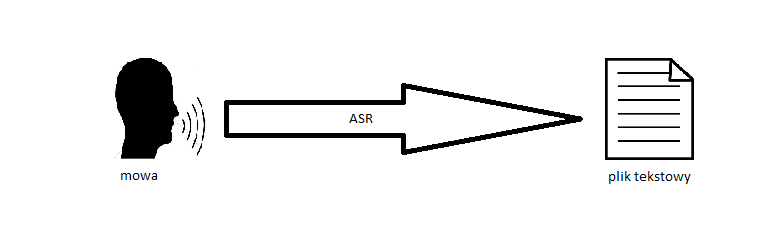
\includegraphics[scale=0.55]{ASRImage.png} }
			\caption{Rozpoznawanie mowy; wejście: mowa -\textgreater wyjście: tekst }\label{fig:hub_and_spoke}
		\end{figure}
	\item synteza mowy, oznaczana jako TTS ( z języka angielskiego Text To Speech)
		\setlength\fboxsep{20pt}
		\setlength\fboxrule{1pt}
		\begin{figure}[!h]
			\centering
			\fbox{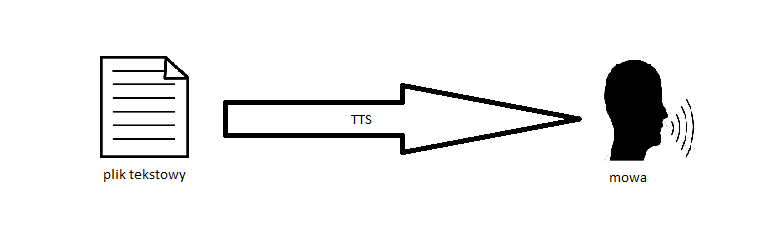
\includegraphics[scale=0.55]{TTSImage.png} }
			\caption{Synteza mowy; wejście: tekst -\textgreater wyjście: mowa}\label{fig:hub_and_spoke}
		\end{figure} 
\newpage
	\item optyczne rozpoznawanie tekstu (tekst można traktować jako zapis mowy), oznaczane skrótem OCR (z języka angielskiego Optical Character Recognition)
		\setlength\fboxsep{20pt}
		\setlength\fboxrule{1pt}
		\begin{figure}[!h]
			\centering
			\fbox{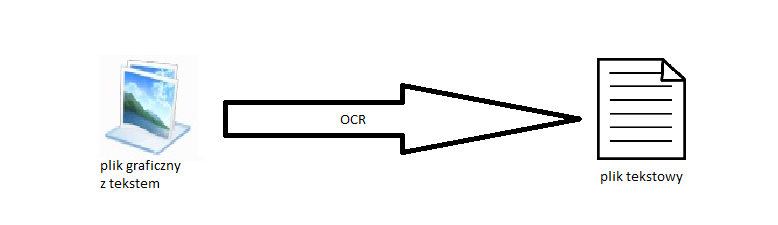
\includegraphics[scale=0.55]{OCRImage.png} }
			\caption{Rozpoznawanie tekstu; wejście: plik graficzny z tekstem -\textgreater wyjście: tekst}\label{fig:hub_and_spoke}
		\end{figure}
	\item tłumaczenie maszynowe mowy
		\setlength\fboxsep{20pt}
		\setlength\fboxrule{1pt}
		\begin{figure}[!h]
			\centering
			\fbox{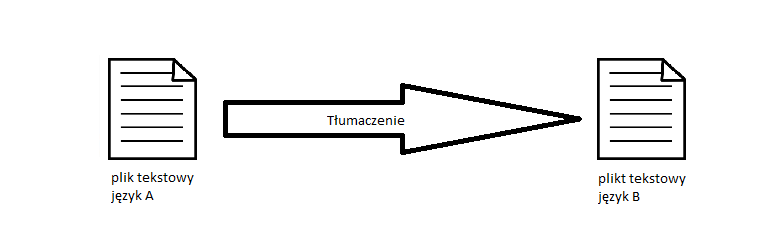
\includegraphics[scale=0.55]{TlumaczenieImage.png} }
			\caption{Tłumaczenie; wejście: tekst -\textgreater wyjście: tekst}\label{fig:hub_and_spoke}
		\end{figure}
\newpage
	\item rozpoznawanie języka
		\setlength\fboxsep{20pt}
		\setlength\fboxrule{1pt}
		\begin{figure}[!h]
			\centering
			\fbox{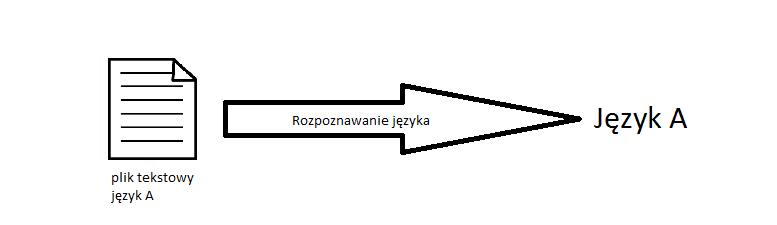
\includegraphics[scale=0.55]{RozpoznawanieImage.png} }
			\caption{Rozpoznawanie języka; wejście: tekst -\textgreater wyjście: informacja o języku tekstu}\label{fig:hub_and_spoke}
		\end{figure}
\end{itemize} 
\subsection{Rozpoznawanie mowy}
Rozpoznawanie mowy jest to proces w wyniku którego komputer wyposażony w odpowiednie oprogramowanie może interpretować ludzką mowę i zamieniać ją na tekst \cite{douglas2002}. Systemy oferujące przetwarzanie mowy można rozróżniać	 według dwóch różnych kryteriów:
\begin{itemize}
	\item sposobu uczenia się
	\item sposobu rozpoznawania mowy
\end{itemize}
Stosując pierwsze kryterium, aplikacje można podzielić na
\begin{itemize}
	\item zależne od lektora
	\item niezależne od lektora
\end{itemize}
Systemy należące do pierwszej grupy uczą się poprzez sesje w czasie których lektor czyta porcje tekstu, aplikacje analizują głos, ton oraz tempo  w efekcie czego mogą dostosować się do danego lektora co skutkuje uzyskaniem o wiele dokładniejszych wyników, w przedziale 95-100\%, oczywiście przy założeniu, że lektor ma podobny głos.  Systemy należące do drugiej grupy uczą się przy wykorzystaniu różnych lektorów. Uzyskiwane przez nie wyniki rzadko przekraczają 75\% jednak są dużo bardziej stabilne, to znaczy nie zależnie od lektora wyniki są w tej okolicy. 
Stosując kryterium drugie wyróżniamy następujące grupy systemów \cite{gaikwad2010} :
\begin{itemize}
	\item Rozpoznające izolowane słowa - są to dość proste systemy, posiadające dwa stany: nasłuchujący i nie nasłuchujący,  wymagające ciszy na początku i na końcu każdej wypowiedzi,  akceptują jedno słowo lub krótką wypowiedź 
	\item Rozpoznające łączone słowa - podobne do systemów z grupy powyżej, charakteryzują się znacznie większą czułością na przerwy pomiędzy kolejnymi słowami czyli umożliwiają osobnym wypowiedziom występować tylko, z minimalnymi przerwami pomiędzy nimi
	\item Rozpoznające mowę ciągłą -  systemy z tej grupy umożliwiają użytkownikowi mówienie w sposób niemal naturalny w czasie gdy one rozpoznają zawartość. Są to najnowsze i najbardziej zaawansowane systemy.
\end{itemize}
\subsection{Synteza mowy}   
Synteza mowy jest wygenerowaną komputerową symulacją ludzkiej mowy. Syntezatory, czyli systemy komputerowe, które dokonują syntezy można podzielić na grupy stosując dwa różne kryteria:
\begin{itemize}
	\item sposób implementacji
	\item sposób tworzenia mowy
\end{itemize}
Systemy należące do pierwszej grupy można podzielić na:
\begin{itemize}
	\item implementowane programowo
	\item implementowane sprzętowo
\end{itemize}
Kategoria pierwsza jest bardziej liczna, łatwiej dostępna, tańsza przez co też dużo bardziej popularna. Dużą zaletą aplikacji należących do pierwszej grupy jest ich uniwersalność,  mogą one być łatwo wykorzystani do różnych celów takich jak:
\begin{itemize}
	\item lektorzy filmowi/e-książek/wiadomości email
	\item poczty głosowe
	\item pomoc techniczna
	\item interaktywna obsługa osoby  dzwoniącej
\end{itemize}
Najpopularniejsze syntezatory mowy dostępne na rynku to:
\begin{itemize}
	\item IvonaTTS
	\item TextAloud
	\item Loquendo
\end{itemize}
Systemy należące do kategorii drugiej (implementowane sprzętowo) charakteryzują się dużo większą wydajnością i szybkością działania. Najlepsze z nich są w stanie generować mowę w czasie rzeczywistym. 
Ze względu na sposób tworzenia mowy, systemy można podzielić na:
\begin{itemize}
	\item Syntezatory artykulacyjne stosują metodę polegającą na kontrolowaniu artykulatorów mowy takich jak szczęka, język, policzki itd. Systemy te próbują modelować mechaniczne ruchy artykulatorów.
	\item Syntezatory korzystające z metody konkatenacyjnej korzystają z dużej bazy oznaczonych próbek(słów) prawdziwego głosu lektora, proces syntezy sprowadza się do wybranie, modyfikacji i konkatenacji tych nagrań. 
	\item Syntezatory alofoniczne, w czasie działania składają potrzebne słowa z dźwięków elementarnych przechowywanych w pamięci i wywoływanych w odpowiedniej chwili. 
\end{itemize}
\subsection{Optyczne rozpoznawanie tekstu}
Optyczne rozpoznawanie tekstu, dużo częściej występujące w wersji skróconej OCR, to mechaniczna lub elektroniczna konwersja obrazu pisma ręcznego lub maszynowego do tekstu przechowywanego w postaci cyfrowej, pozwalającej na dalszą jego obróbkę. Podobnie jak w przypadku syntezatorów mowy systemy OCR można podzielić na:
\begin{itemize}
	\item implementowane programowo
	\item implementowane sprzętowo
\end{itemize}
Podobnie jak przy syntezatorach zaletą implementacji sprzętowej jest szybkość oraz wydajność co umożliwia pracę w czasie rzeczywistym. Niezależnie od implementacji, sposób ich działania oraz algorytmy pozostają podobne. Podstawowe kroki jakie system musi podjąć w celu rozpoznania tekstu to \cite{noor2005} :
\begin{enumerate}
	\item Wczytanie obrazu jako mapy bitowej z podanego źródła.
	\item Rozpoznanie najważniejszych cech obrazu takich jak rozdzielczość i inwersja. Wiele algorytmów spodziewa się kolorów i rozmiaru czcionki w ramach wcześniej zdefiniowanego przedziału dlatego też obraz musi być przeskalowany i znormalizowany przed dalszą obróbką. Na tym etapie rozpoznawane również są pozycje i typy najważniejszych części obrazu.
	\item Wiele algorytmów wymaga by obraz był dwukolorowy, dlatego kolorowy albo szary obraz musi być przekonwertowany do biało czarnej postaci, to bardzo istotny krok algorytmu ponieważ błędy w tej części mogą powodować poważne problemy w dalszych etapach.
	\item Kolejnym ważnym krokiem jest usunięcie wszystkich podkreśleń, obramowań itd. w dalszej kolejności umożliwia to rozpoznanie linii tekstu co jest jednym z kluczowych kroków poprawnego algorytmu.
	\item Po podzieleniu tekstu na linie, algorytm stara się rozpoznać błędne znaki, to znaczy takie które stykają się z innymi albo są podzielone na kilka części (np. w wyniku konwersji do biało czarnej postaci), i je dopasować do znanej mu puli.
	\item Ostatnim i najważniejszym krokiem jest rozpoznanie pojedynczych znaków, sukces tego kroku zależy od poprzednich etapów. Najpierw każdemu znakowi próbuje się dopasować kod znaku, czasami nie jest możliwe dopasowanie tylko jednego kodu, np. w przypadku litery \textbf{I} większość algorytmów rozpozna ją jako \textbf{I}, \textbf{|}, \textbf{1} lub \textbf{i}. W takim przypadku należy skorzystać ze słownika, posiadanie bogatej bazy słów, może, w sposób znaczący poprawić efektywność algorytmu.
\end{enumerate}
Nie jest to kompletna lista kroków, istnieje dużo innych mniejszych lub większych etapów, jednak każdy z wymienionych jest bardzo ważny, cały proces nie zakończy się sukcesem jeżeli zawiedzie którykolwiek z nich. 
\subsection{Translacja mowy}
Translacja mowy to tłumaczenie z jednego języka na inny. Aplikacje tłumaczące często nazywane są translatorami. Mimo, że z pozoru mogłoby się wydawać, że jest to czynność prostsza niż OCR czy też ASR to tak nie jest. Proces tłumaczenia jest bardzo trudny i do tej pory nie istnieją aplikacje nie popełniające błędów. W zasadzie można wyróżnić trzy typy translatorów, bazując na algorytmach jakie stosują co do tłumaczonego tekstu:
\begin{itemize}
	\item algorytmy oparte na zasadach gramatyki
	\item algorytmy bazujące na podejściu statystycznym
	\item algorytmy stosujące translacje opartą o przykłady
\end{itemize}
W podejściu pierwszym przeprowadza się tłumaczenie bazując na informacjach językowych na temat języka źródłowego i docelowego. Algorytm rozkłada zdanie na części pierwsze, analizuje je, następnie bazując na bazie wiedzy którą posiada, a w skład której wchodzą informacje na temat składni, budowy zdań, odmian oraz słownik dwujęzyczny, buduje zdanie w języku docelowym. Technika ta wymaga ogromnej mocy obliczeniowej oraz dużych zasobów danych, według ekspertów w dziedzinie translacji, takich jak Franz Josef Och \cite{och2003}, jest nieefektywna.
W podejściu statystycznym tłumaczenia dokonuje się w oparciu o statystyczny model którego parametry są wyliczane na podstawie analizy tekstu. Jest do podejście mające bardzo mocne oparcie w teorii informacji. W chwili obecnej wydaje się, że jest ono najbardziej efektywne o czym może świadczyć fakt, że podejście to zostało zastosowane przez Google przy tworzeniu Google Translator, który wygrał międzynarodowe zawody w tłumaczeniu z angielskiego na arabski i angielskiego na chiński.
Stosowanie algorytmów opartych o analogie jest najprostszym z możliwych podejść, może być postrzegane jako implementacja uczenia maszynowego w podejściu CBR \footnote{http://www.ai-cbr.org/classroom/cbr-review.html}. Uważa się, że podejście to najbardziej dokładnie oddaje proces myślowy człowieka tłumaczącego tekst, to znaczy najpierw następuje dekompozycja zdania na mniejsze frazy, następnie tłumaczy się te frazy pojedynczo i odpowiednio łączy tworząc zdanie w języku docelowym. Translator bazujący na takim podejściu musi przejść fazę uczenia, polegającą na podawaniu na wejście podobnych zdań w dwóch językach różniących się tylko nieznacznie. Stosując dwa proste zdania w językach angielski i japońskim: 
 \begin{itemize}
	\item ang: \verb"How much is that red umbrella?" jap: \verb"Ano akai kasa wa ikura desu ka?"
	\item ang: \verb"How much is that small camera?" jap: \verb"Ano chiisai kamera wa ikura desu ka?"
\end{itemize} 
system nauczy się, że:
 \begin{enumerate}
	\item \verb"How much is X?" odpowiada \verb"Ano X wa ikura desu ka?"
	\item \verb"red umbrella" odpowiada \verb"akai kasa"
	\item \verb"small camera" odpowiada \verb"chiisai kamera"
\end{enumerate} 
Następnie aplikacja może zastosować w ten sposób nabytą wiedzę w bardziej zaawansowanych przypadkach.
\subsection{Rozpoznawanie języka}
Rozpoznawanie języka \cite{adamsresnik1997}  to proces którego celem jest stwierdzenie w jakim języku naturalnym jest podana na wejście próbka tekst lub mowy. Praca ta skupia się na rozwiązaniach rozpoznających język tekstu. Tradycyjne podejście, stosowane np. w księgarniach, opiera się na zidentyfikowaniu najczęściej występujących słów i liter które są charakterystyczne dla danego języka i sprawdzenie ich w odpowiednich tabelach. Implementacja algorytmów działających na podobnej zasadzie jest możliwa jednak jest to rozwiązanie mało efektywne. Obecnie stosuje się kilka różnych podejść bazujących na statystyce:
 \begin{itemize}
	\item Bardzo prostą techniką jest porównywanie jakości kompresji badanego tekstu z jakością kompresji tekstów w znanych językach, im bardziej zbliżone wyniki tym większe prawdopodobieństwo, że teksty są w tym samym języku. Podejście to nazywa się miarą odległości wzajemnej informacji.
	\item Bardziej zaawansowanym algorytmem jest ten zaproponowany przez W.Cavnar'a i J.Trenkle'a w 1994 roku pod nazwą: ''N-Gram-Based Text Categorization''. Najpierw należy utworzyć znakowy n-gramowy model języka na podstawie materiałów treningowych dla każdego z języków które mają być obsługiwane. Następnie dla każdego tekstu którego język ma być zidentyfikowany, tworzy się podobny model i porównuje z modelami bazowymi. Im bardziej są do siebie podobne tym większa szansa, że to ten sam język. Problematyczne w tym podejściu są języki dla których nie można skonstruować takiego modelu. 
	\item Rozszerzeniem poprzedniego algorytmu jest technika zaproponowana przez Rehurka i Kolkusa \cite{rehurek2009} . Największymi zaletami ulepszonej wersji jest fakt, że nie zawodzi ona w sytuacji w której próbka tekstu jest napisana w wielu językach, a także nie stanowi dla niej problemu rozróżnianie języków należących do tej samej rodziny (np. polski i słowacki). 
\end{itemize} 
Jak widać przetwarzanie mowy samo w sobie jest bardzo obszernym i skomplikowanym tematem, w skład którego wchodzi wiele różnych procesów które można zintegrować tworząc efektywne i bardzo funkcjonalne systemy.

\section{Paradygmat SOA}
SOA czyli Service Oriented Architecture(Architektura zorientowana na usługi) to zgodnie z definicją zaproponowaną przez W3C zbiór komponentów dostępnych w sieci posiadających dobrze opisane interfejsy. Opis ten pozwala na rozróżnianie komponentów i ich wyszukiwanie, a następnie wywoływanie. Najbardziej popularną obecnie implementacją tego paradygmatu jest ta opierająca się o technologię web services.  W paradygmacie SOA możemy wyróżnić dwa różne podejścia tworzenia złożonych usług:
 \begin{itemize}
	\item orkiestracja
	\item choreografia
\end{itemize}  
Orkiestracja charakteryzuje się tym, iż istnieje jedna usługa orkiestrator, dyrygent lub koordynator który zarządza innymi usługami w celu udostępniania jednej funkcjonalności. Prowadzi to do luźniejszego połączenia usług, sprawia też, że nie są one świadome bycia częścią większego procesu. Orkiestracja jest scentralizowaną formą współpracy z dobrze zdefiniowanymi operacjami i kolejnością wywoływania usług. Istnieją specjalne języki, ułatwiające taką integrację usług, na przykład BPEL.
\begin{figure}[!h]
	\centering
	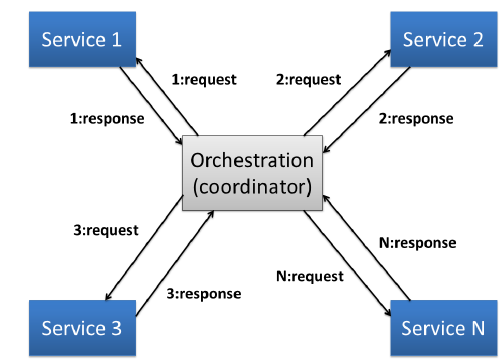
\includegraphics[scale=0.75]{orkiestracja.png} 
	\caption{Orkiestracja}
\end{figure}
\newpage
Choreografia to sposób współpracy usług, charakteryzujący się tym,  iż każda z nich musi być świadoma bycia częścią czegoś większego, od niej zależy kiedy i z kim się skomunikuje. Nie ma tutaj centralnego zarządzania, koordynatora czy też usługi nadrzędnej. 
\begin{figure}[!h]
	\centering
	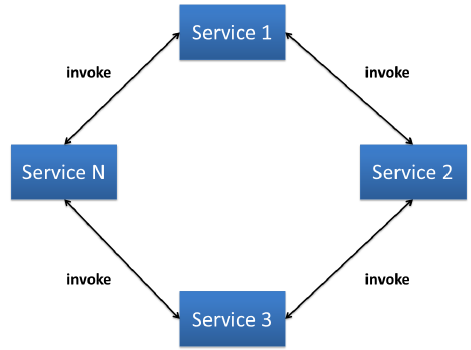
\includegraphics[scale=0.75]{choreogragia.png} 
	\caption{Choreografia}
\end{figure}

\section{Sposoby integracji systemów komputerowych}
Dzięki postępowi technologicznemu przepustowość łączy internetowych wciąż wzrasta powodując, bardzo szybki rozwój systemów komputerowych i usług przez nie oferowanych. Powstają nowe rodzaje usług, które kiedyś nie mogły by zostać zrealizowane, przy tworzeniu zaś niektórych aplikacji, to co kiedyś było problemem i na czym skupiali swój wysiłek twórcy oprogramowania, dzisiaj schodzi na drugi plan. Z drugiej jednak strony zwiększają się wymagania użytkowników co do jakości, są wprowadzane coraz to nowe formaty, które wymagają ogromnych przepustowości, przez co mogą zapychać łącza i tworzyć opóźnienia. Jest to szczególnie istotne w systemach czasu rzeczywistego, w których nacisk na jak najmniejsze opóźnienia jest bardzo silny. Czasami jednak aplikacje i ich użytkownicy nie mają takich ścisłych wymagań co do wielkości opóźnienia. W ich przypadku opóźnienie nawet rzędu kilkudziesięciu sekund nie stanowi problemu i jest akceptowalne przez użytkowników. W takim wypadku nie trzeba się skupiać na szukaniu idealnego rozwiązania dla danego problemu, lecz można skupić się na stworzeniu architektury która ułatwi i przyspieszy budowanie systemów spełniających dane wymagania.

Przy takim podejściu do tworzenia systemu zazwyczaj pojawia się problem integracji budowanego systemu z istniejącymi już usługami. Często też, budowany system jest całkowicie problemem integracyjnym, czyli wszystkie składowe usługi potrzebne do realizacji celu biznesowego są dostępne, a jedyne zadanie stawiane budowanemu systemowi to odpowiednia integracja tych usług. Podejście takie ułatwia parę kwestii, ale w zamian wprowadza także nowe, specyficzne dla siebie problemy. Głównym problemem jest różnorodność dostępnych podsystemów. Każdy z nich może być stworzony przy użyciu innych technologii (Java, COM, .Net, CORBA, ICE, itp.) działać na innej platformie (MS WINDOWS, LINUX, SOLARIS) i co najważniejsze mogą wykorzystywać inne protokoły do komunikacji (RPC, SOAP, własnościowe protokoły, itp). Z tego powodu decyzja o sposobie integracji nie może być podejmowana zbyt szybko,  powinna być podjęta bazując na pewnych kryteriach:  \cite{hohpewoolf2003} 

\begin{itemize}
	\item \textbf{powiązanie aplikacji} - integracja aplikacji powinna minimalizować powiązania i zależności między nimi, co pozwoli na swobodne rozwijanie każdej aplikacji z osobna. Ściśle powiązane aplikacje współdziałają przy wielu założeniach z każdej ze stron. Jeżeli któraś z aplikacji zostanie zmieniona i założenia co do niej nie będą już spełnione wtedy cały system przestanie działać. Dlatego też, projektowane interfejsy powinny być na tyle specyficzne aby umożliwiały implementacje użytecznych funkcjonalności, lecz także na tyle ogólne aby umożliwiały zmianę implementacji, jeżeli zajdzie taka potrzeba.
	\item \textbf{poziom ingerencji} - podczas integracji aplikacji, powinno się minimalizować zarówno zmiany w samej aplikacji jak i ilość kodu tworzonego na rzecz integracji. Jednak bardzo często zarówno zmiany w aplikacji jak i tworzenie dodatkowe kodu odpowiadającego za integracje jest nieuniknione aby uzyskać odpowiednią funkcjonalność. Rozwiązania mniej ingerujące w aplikacje mogą nie zapewniać integracji w odpowiednim stopniu.
	\item \textbf{wybór technologii} - do wyboru mamy mnóstwo technologii integracyjnych, które różnią się od siebie wymaganiami zarówno co do specjalistycznego sprzętu jak i oprogramowania. Niektóre z nich są wymienne między sobą, natomiast wybranie innych może doprowadzić do zamknięcia się na dane rozwiązanie. Jeżeli podejmie się decyzję o zastosowaniu którejś z gotowych technologii integracyjnych może ona znacząco zwiększyć koszt całego system. Z drugiej strony, integracja od podstaw zazwyczaj kończy się większym nakładem pracy niż początkowo planowano i może oznaczać odkrywanie koła na nowo.
	\item \textbf{format danych} - integrowane aplikacje muszą posługiwać się tym samym formatem podczas wymiany danych. Dostosowywanie istniejących aplikacji do jednolitego formatu danych może być bardzo trudne, albo wręcz nie możliwe. Inną opcją jest wprowadzenie elementu pośredniego, którego celem będzie tłumaczenie danych z jednego formatu na drugi. Problemem powiązanym z opisanym w tym podpunkcie jest rozszerzalność i rozwój formatu danych - jak może się zmieniać z biegiem czasu i jak te zmiany wpłyną na aplikacje.
	\item \textbf{żywotność danych} - integracja powinna minimalizować czas pomiędzy udostępnieniem danych przez jedną aplikację, a pobraniem tych danych przez drugą aplikacje. Można to osiągnąć poprzez częstą wymianę małych porcji danych, jednakże takie podejście może zmniejszyć wydajność całego systemu. Opóźnienia związane z wymianą danych muszą zostać wzięte pod uwagę podczas planowania integracji. W idealnym systemie, aplikacja odbiorcza zostanie poinformowana jak tylko dane będą dostępne. Im dłuższy czas miedzy publikacją a konsumpcją danych tym większa szansa, że aplikacje ulegną rozsynchronizowaniu.
	\item \textbf{rodzaj komunikacji} - przetwarzanie komputerowe jest w dużej mierze synchroniczne - to znaczy, że jedna procedura wywołuje drugą ( podprocedurę) i czeka na jej wykonanie. W systemach rozproszonych, wywołania mają charakter zdalny, co powoduję, że są o wiele wolniejsze od wywołań lokalnych. Z tego powodu, oczekiwanie na zakończenie wywołania, jest często niepożądane. W takim wypadku można wykorzystać podejście asynchroniczne - procedura wywołująca podprocedurę, lecz nie czeka na jej zakończenie, tak jak to było przy wywołaniu synchronicznym, tylko wraca do swojego przetwarzania. Kiedy podpprocedura zakończy przetwarzanie, informuję o tym procedurę wywołująca i zwraca jej wynik. Komunikacja asynchroniczna może zwiększyć wydajność całego systemu, ale również może uczynić go bardziej złożonym.
	\item \textbf{poziom niezawodności} - komunikacja zdalna jest nie tylko wolniejsza, ale również bardziej zawodna niż lokalne wywołania funkcji. Kiedy procedura wywołuje podprocedurę w obrębie jednej aplikacji, jest pewne, że ta podprocedura jest dostępna. Takie założenie nie musi być spełnione jeżeli chodzi o zdalne wywołania - zdalna aplikacja może nie działać w chwili wywołania, albo połączenie z siecią może być tymczasowo niedostępne.
\end{itemize}

Do wyboru mamy wiele różnych technologii integracyjnych. Niektóre z nich są niezależne od platformy, inne zaś wymagają specyficznego systemu operacyjnego. Jedne są darmowe i otwarte, inne zaś płatne i oparte na własnościowych patentach i protokołach. Każda z nich ma swoje plusy i minusy dlatego trzeba wybrać tą która najlepiej nadaje się dla określonego celu. Dodatkową opcją jest tworzenie swojego systemu integracji od zera. Jednak rozwiązanie takie jest czasochłonne, kosztowne a także jego celowość stoi pod znakiem zapytania więc bardzo często nie jest ono brane pod uwagę.
Dostępne rozwiązania można podzielić na cztery grupy: \cite{chappell2004}

\begin{itemize}
	\item serwery aplikacji
	\item EAI brokers
	\item dedykowane rozwiązania MOM
	\item ESB
\end{itemize}
\setlength\fboxsep{20pt}
\setlength\fboxrule{1pt}
\begin{figure}[!h]
	\centering
	\fbox{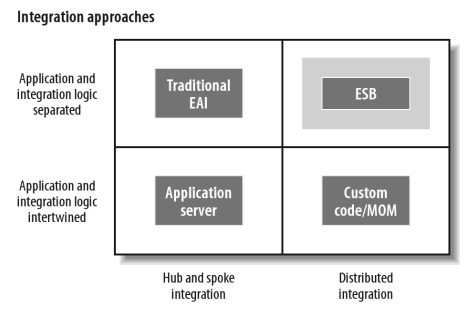
\includegraphics{podejscia_integracyjne.png} }
	\caption{Różne podejścia integracyjne  \cite{chappell2004}}\label{fig:podejscia_integracyjne}
\end{figure}

Pierwsze dwie grupy rozwiązań oparte są na modelu \textbf{"Hub and Spoke"}  w modelu tym połączenia ułożone są na wzór koła rowerowego, w którym przebieg danych odbywa się wzdłuż szprych (spoke) połączonych z położoną w centrum piastą (hub). Zaletą takiego rozwiązania jest scentralizowanie takich funkcji systemu jak: zarządzanie, routowanie wiadomości, logika biznesowa, które to są zaimplementowane w węźle centralnym (hub). Dzięki temu poszczególne elementy integrowane są wyposażone tylko w niezbędną dla nich funkcjonalność. Kolejną zaletą jest ilość połączeń którą trzeba zrealizować w takim modelu. Przy założeniu, że tworzymy \begin{math}n\end{math}  systemów i każdy z nich musi komunikować się z resztą to suma połączeń które trzeba zrealizować wynosi  \begin{math}n\end{math}  złożoność powstałej sieci wynosi  \begin{math}O(n)\end{math}  Jak widać ostateczna złożoność jest znacznie lepsza niż przy połączeniach punk-punkt miedzy każdym systemem. Przy połączeniach system-system  ilość potrzebnych połączeń wynosi   \begin{math}\frac{n (n- 1)}{2}\end{math}  Złożoność takiej sieci połączeń wynosi  \begin{math}O(n^2)\end{math}  Wadami takiego rozwiązania jest słaba skalowalność, istnienie pojedynczego punktu awarii w postaci węzła centralnego(hub) oraz wprowadzenie dodatkowego opóźnienia, a mianowicie jednego dodatkowego przeskoku w porównani z komunikacją system-system).

\setlength\fboxsep{20pt}
\setlength\fboxrule{1pt}
\begin{figure}[!h]
	\centering
	\fbox{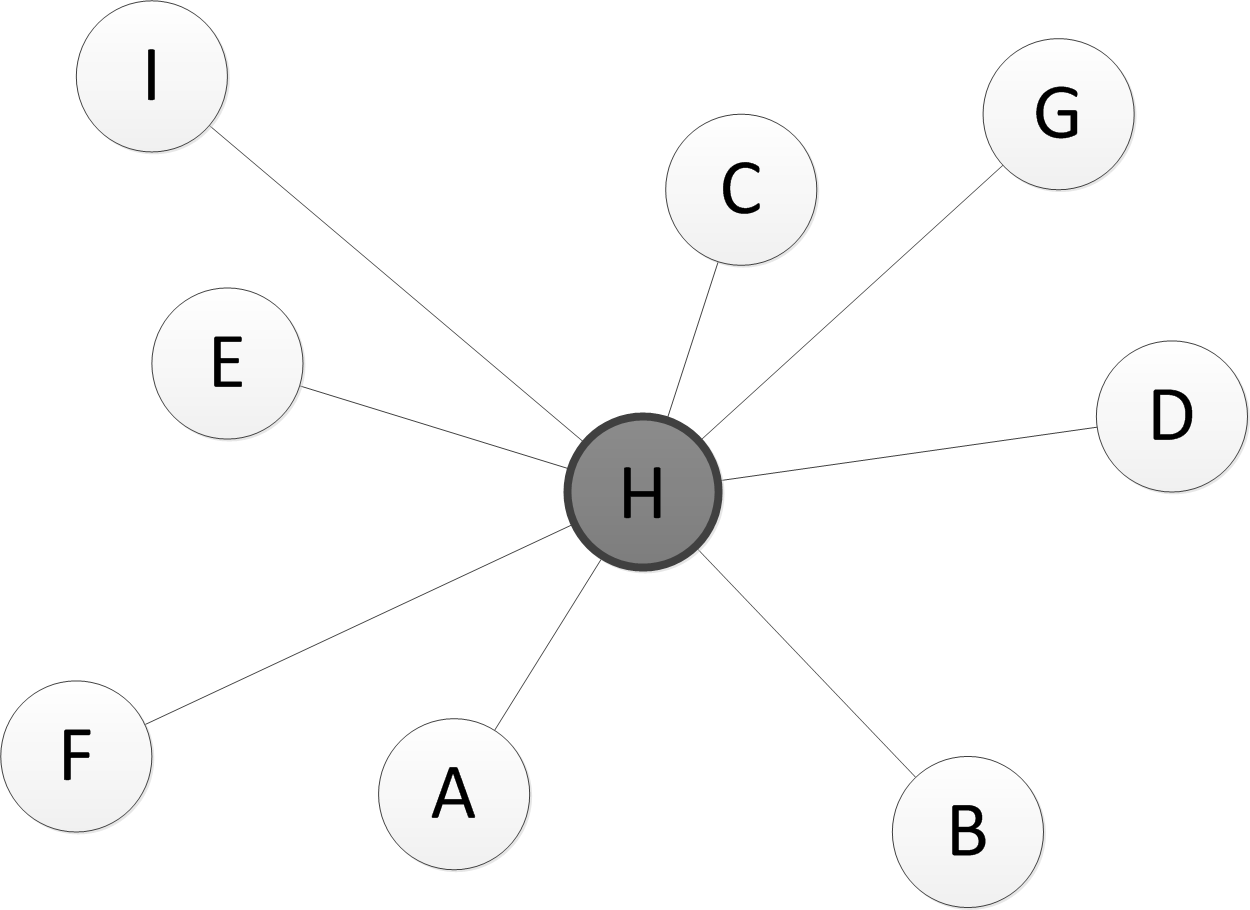
\includegraphics[scale=0.24]{hub_and_spoke_model.png} }
	\caption{Model "Hub and spoke"}\label{fig:hub_and_spoke}
\end{figure}

Rozwiązania oparte na serwerach aplikacji upraszczają implementację komunikacji ponieważ serwery te zazwyczaj są wyposażone w obsługę standardowych protokołów takich jak HTTP czy SOAP. Minusem tych rozwiązań jest to, że logika integracyjna i logika biznesowa przeplatają się nawzajem, a także poszczególne części systemu są dość mocno ze sobą powiązane co zmniejsza elastyczność systemu.

EAI brokers wypadają lepiej od serwerów aplikacji ponieważ rozdzielają logikę integracyjną od logiki biznesowej. Jednak rozwiązanie to posiada wszystkie wady związane z modelem hub and spoke na którym jest oparte.

Rozwiązania bazujące na MOM pozwalają na luźne łączenie poszczególnych systemów a także na asynchroniczną komunikację między nimi. Rozwiązania te zazwyczaj nie posiadają wysoko poziomowej warstwy abstrakcji nad logiką routowania co fragmentami wymusza programowanie na dość niskim poziomie. Z tego też powodu, rozwiązania te, podobnie jak rozwiązania oparte na serwerach aplikacji cierpią z powodu przeplatającej się logiki integracyjnej z logiką biznesową, co utrudnia utrzymywanie i rozwijanie takiego systemu.

Ostatnia grupa rozwiązań jest oparta na ESB. Jest to zdecydowanie najnowsza z wyżej opisanych technologii. Dzięki doświadczeniu zdobytemu przy użytkowaniu poprzedników, udało się stworzyć technologię, która nie posiada tych samych wad. Ogólnie rzecz ujmując ESB dostarcza warstwę abstrakcji opartą na implementacji biznesowego systemu wymiany wiadomości, dzięki temu pozwala wykorzystać zalety wiadomości bez pisania dodatkowego kodu. W przeciwieństwie do bardziej klasycznego podejścia (EAI) opartego o architekturę hub and spoke podstawa platformy jest zbudowana z funkcji bazowych podzielonych na części składowe które mogą być osadzane zarówno w jednolitym jak i rozproszonym środowisku wzajemnie ze sobą współpracując. Szkielet ESB do zarządzania usługami wykorzystuje komunikację działającą w oparciu o asynchroniczne przesyłanie wiadomości, ten sam system jest wykorzystywany do komunikacji pomiędzy usługami osadzonymi w kontenerze. Najważniejszą cechą ESB jest fakt, iż po wpięciu aplikacji przez ściśle zdefiniowany, bazujący na standardach interfejs, uzyskuje ona dostęp do całej infrastruktury i usług udostępnianych przez ESB a także do każdej innej, już działającej aplikacji. W chwili obecnej dostępnych jest wiele różnych implementacji ESB, większość z nich udostępnia podobne usługi więc ciężko je stosować jako kryterium, lepszym sposobem by rozróżnić implementacje jest zastosowanie następującej miary:
\begin{itemize}
	\item wspierane środowisko działania/osadzania
	\item model kontenera - bazujący na standardach czy własnościowy
	\item powiązanie z innymi elementami architektury
	\item zależności
\end{itemize}
Co równie ważne, wszystkie implementacje ESB oferują również bardzo wiele różnych rodzajów punktów końcowych. Umożliwiają one bardzo łatwe pobieranie danych z różnych źródeł, takich jak:
\begin{itemize}
	\item mail
	\item ftp
	\item technologia web services
	\item technologia REST web services
	\item RSS
\end{itemize}

\section{Integracja systemów przetwarzania mowy}

Podrozdział ten ma na celu przedstawić  jakie wymagania można postawić przed przykładową aplikacją integrującą systemy przetwarzania mowy i jak wpłyną one na sposób integracji. Aby zdefiniować wymagania można rozważyć przykładową aplikację kliencką która mogłaby być zbudowana w oparciu o taki system. Podstawowe funkcje, które taka aplikacja realizuje mogą być następujące:
\begin{itemize}
	\item zamiana pliku graficznego będącego zdjęciem tekstu na plik tekstowy (OCR)
	\item synteza tekstu (TTS)
	\item tłumaczenie tekstu 
	\item zamiana mowy na tekst (ASR)
	\item rozpoznanie języka tekstu - jest to specjalny przypadek, od wymienionych wyżej różni się tym, że nie przetwarza tekstu w dosłownym tego słowa znaczeniu, co prawda na wejściu potrzebny jest tekst, jednak na wyjściu otrzymujemy informację o nim, a nie jego przetworzoną wersję
\end{itemize}
Oczywiście każde z wyżej wymienionych zadań może zostać zrealizowane osobno przez odpowiednie aplikacje. Dlatego, gotowy system powinien być w stanie realizować każdą z nich osobna jak i każdą możliwą i sensowną kombinację. Dobrym przykładem takiej złożonej funkcjonalności jest zamiana pliku w formacie graficznym, będącym zdjęciem np. strony książki(napisanej w nieznanym języku) na dźwięk w jakimś innym, konkretnym, zdefiniowanym przez użytkownika języku. Aby to osiągnąć należy poinformować system o tym z których usług należy skorzystać i w jakiej kolejności je wywołać. Oczywiście idealnym i na szczęście możliwym rozwiązaniem jest ukrycie całej implementacji za jednym prostym interfejsem. Jednym z przykładowych rozwiązań tego problemu może być plik konfiguracyjny (na przykład w formacie xml) wysyłany razem z danymi wejściowymi. Przykładowa struktura takiego pliku mogłaby wyglądać następująco:
 \begin{itemize}
	\item \textless speechProcessingInstructions\textgreater - podstawowy element, będący korzeniem dla całego pliku
	\item \textless readImage\textgreater - wystąpienie tego elementu oznacza, że na wejściu należy oczekiwać pliku graficznego, zawierającego tekst, na którym zostanie wywołana usługa OCR, w efekcie czego powstanie plik tekstowy
	\item \textless identifyLanguage\textgreater - element oznaczający konieczność użycia usługi rozpoznającej język, na wejściu oczekującej pliku tekstowego, zwracającej informację o języku
	\item \textless translate\textgreater - element wymuszający użycie translatora, na wejściu oczekuje pliku tekstowego, zwraca plik tekstowy, posiada następujące węzły potomne:
		 \begin{itemize}
			\item \textless inputLanguage\textgreater - element, którego zastosowaniem jest zdefiniowane języka tekstu wejściowego, jeżeli operacją poprzednią  było rozpoznanie języka element ten zostanie pominięty
			\item \textless outputLanguage\textgreater - element, którego zastosowaniem jest zdefiniowane języka tekstu docelowego
		\end{itemize}
	\item \textless performTTS\textgreater - element oznaczający konieczność wywołania usługi odpowiadającej za syntezę mowy, na wejściu oczekującej pliku tekstowego, zwracającej plik dźwiękowy
	\item \textless performASR\textgreater - wystąpienie tego elementu oznacza użycie usługi odpowiedzialnej  za rozpoznawanie mowy, przyjmuje ona plik dźwiękowy, zwraca plik tekstowy
\end{itemize}
Zastosowanie takiego formatu ma dużo zalet, z czego najważniejsze to:
\begin{itemize}
	\item prostota
	\item duża ilość narzędzi wspierających ten format
	\item popularność w środowisku SOA
	\item czytelność dla człowieka
	\item łatwa rozbudowa
\end{itemize}
\newpage
Przykładowy plik konfiguracyjny potrzebny do realizacji opisanego wyżej scenariusza wyglądałby następująco:

\setlength\fboxsep{20pt}
\setlength\fboxrule{1pt}
\begin{figure}[!h]
	\centering
	\fbox{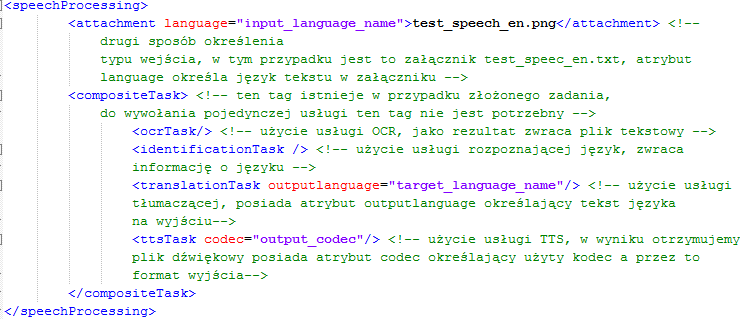
\includegraphics[scale=0.8]{sampleXML.png} }
	\caption{Przykładowy plik XML}
\end{figure}

Podsumowując, zakładając istnienie tak działającego systemu, jedyne zadania stawiane przed użytkownikami to:
\begin{itemize}
	\item wygeneriwanie pliku sterującego XML
	\item opcjonalne (zależnie od scenariuszu) przesłanie pliku graficznego do systemu
	\item opcjonalne (zależnie od scenariuszu) przesłanie pliku dźwiękowego go do systemu
	\item pobranie rezultatu działania systemu (np. plik z przetłumaczonym tekstem, plik dźwiękowy, strumień dźwięku itd.)
\end{itemize}
Jak widać są to rzeczy dość proste i możliwe do bardzo szybkiej implementacji. Oczywiście bardzo łatwo można wyobrazić sobie możliwości rozbudowy takiej platformy. Jednym z kierunków takiej rozbudowy może być chęć wykorzystania innych, niż opisane wyżej(plik graficzny, plik xml) formatów danych wejściowych.  Bardzo pomocne okażą się tutaj punkty końcowe, które są oferowane w bardzo wielu różnych rodzajach, tak jak to zostało opisane wyżej, przez wszystkie implementacje ESB. Łatwo wyobrazić sobie użycie punktów końcowych, można je na przykład wykorzystać aby umożliwić użytkownikowi dostęp do usługi drogą mailową. Wystarczy aby użytkownik wysłał na specjalny, oficjalny, podany mu wcześniej adres, maila zawierającego, w postaci załączników, plik sterujący xml oraz plik wejściowy, na przykład zdjęcie tekstu albo tekst, w efekcie czego otrzymałby maila zwrotnego z danymi uzyskanymi w wyniku wykonania żądanych przez niego operacji. Innym przykładem użycia punktów końcowych, w celu zwiększenia funkcjonalności systemu, mogłoby być rozbudowanie pliku sterującego na przykład o tag \textless rssSource\textgreater który sprawi, że aplikacja zamiast pliku wejściowego pobierze wiadomości ze źródła RSS i na nich wywoła funkcje udostępniane przez różne usługi. Jak widać wykorzystanie punktów końcowych daje wiele możliwości i idealnie wkomponowuje się w dziedzinę problemu, co stanowi kolejny argument na rzecz wykorzystania ESB jako sposobu integracji.

\section*{Podsumowanie}
Biorąc pod uwagę proponowane usługi, format danych wejściowych i wymagania stawiane przed platformą zdecydowanie najlepszym sposobem integracji wydaje się wykorzystanie jednej z istniejących implementacji ESB. Wszystkie one zapewniają routing, dużo różnych rodzajów punktów końcowych, wsparcie dla aplikacji pisanych przy użyciu technologii Spring i wiele innych rzeczy które nie tylko ułatwiają sam proces integracji ale również zapewniają możliwość łatwej rozbudowy w przyszłości.



%ksiazka ESB strony 4,5 

%opiszemy to podejscie i potem opiszemy, ze jest bardzo fajne, opiszemy rodzaje, jak ewoluowało, i na koncu opiszemy esb, a potem konkrety dla naszej aplikacji. Obrazki w ksiazce ESB
%ESB strona 34 - czemu własnościowe rozwiązania sa do dupy 



%\subsection {Szyna} 

%Przedstawienie jak to wyglada( kropki serwisy , komunikują sie z roznymi innymi serwisami, dodatokwe serisy: accounting itd)

%Wymagania stawiane rozwiazaniom integracyjnym , Czy warto integrować ? (book1.pdf chapter 2)

%Integracja systemow multimedialnych ??

%Rozwiazania ?

%Brak integracji

%integracja EAI - hub and spikes (scentralizowany punk, single point of failure. słabo scalowalne)

%SOA - ESB 




%service activator (request od clienta)


% ---------------------------------------------------------------------------
%: ----------------------- end of thesis sub-document ------------------------
% ---------------------------------------------------------------------------


% this file is called up by thesis.tex
% content in this file will be fed into the main document
\ifpdf
    \graphicspath{{3/figures/PNG/}{3/figures/PDF/}{3/figures/}}
\else
    \graphicspath{{3/figures/EPS/}{3/figures/}}
\fi
\chapter{Wykorzystane technologie} % top level followed by section, subsection


% ----------------------- contents from here ------------------------
W rozdziale tym, zostaną zaprezentowane oraz po krótce opisane najważniejsze technologie wykorzystane przy implementacji systemu SpeechProcessingPlatform. Rysunek \ref{fig:architecture_and_technologies} przedstawia w której części systemu wykorzystywane są poszczególne technologie.

\begin{figure}[!h]
	\centering
	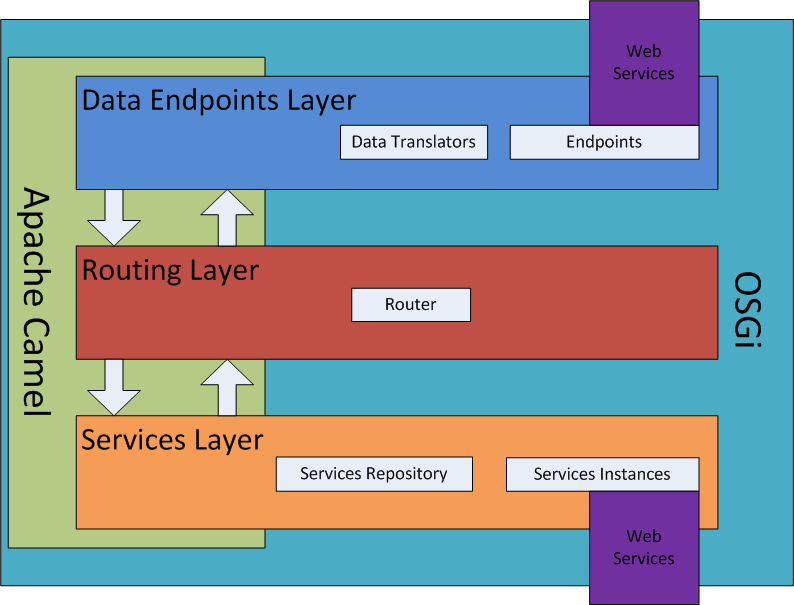
\includegraphics[scale=0.45]{layered_architecture_and_technologies.png} 
	\caption{Architektura systemu SpeechProcessingPlatform wraz z wykorzystywanymi technologiami.}
\label{fig:architecture_and_technologies}
\end{figure}

\section{Technologie integracyjne}
\subsection{OSGi}
Technologia OSGi to zbiór specyfikacji definiujących dynamiczne środowisko komponentowe. Taka struktura pozwala na tworzenie aplikacji złożonych z wielu, różnych komponentów(paczek) które mogą być wykorzystywane wiele razy. Specyfikacja OSGi pozwala komponentowi na ukrywanie swojej implementacji przed innymi i komunikację tylko przy użyciu specjalnych usług, które są dzielone pomiędzy wszystkimi komponentami. Pozwala to na zmniejszenie złożoności tworzonych systemów.

OSGi posiada architekturę warstwową, przedstawiona jest ona, wraz z krótkim opisem, na poniższym diagramie.
\begin{figure}[!h]
	\centering
	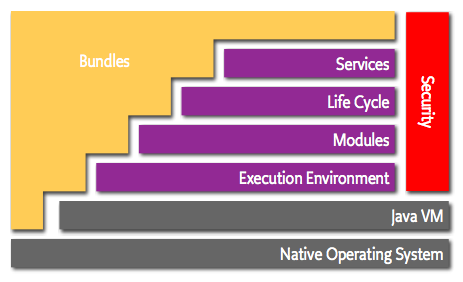
\includegraphics[scale=0.65]{osgiArchitektura.png} 
	\cite{fusehomepage2012}
	\caption{Architektura OSGi}
\end{figure}
\begin{itemize}
	\item Bundles - Są to paczki technologii OSGi, mogą być preinstalowane jak i tworzone i dynamicznie ładowane przez programistów
	\item Services - Warstwa usług dynamicznie łączy komponenty, stosując model publish-find-bin
	\item Life-Cycle - API do startowania, zatrzymywania, instalowania i usuwania komponentów
	\item Modules - Warstwa definiująca jak komponenty mogą importować i eksportować kod	
	\item Security - Warstwa zajmująca się bezpieczeństwem
	\item Execution Environment - Warstwa definiująca jakie metody i klasy są dostępne na specyficznej plarformie
\end{itemize}  
Najważniejszą ideą umożliwiającą istnienie i działanie takiej platformy jest modułowość, której ucieleśnieniem są paczki. OSGi ukrywa wszystko co znajduje się w takim komponencie poza funkcjonalnością która jest wyspecyfikowana. Jeżeli jeden komponent chce wykorzystać inny musi wyraźnie definiować jaką funkcjonalność potrzebuje. Ponieważ ciężko stworzyć model współpracy opierając się tylko na klasach, OSGi wprowadza warstwę usług, a wraz z nią rejestr konkretnych usług. Paczka może stworzyć obiekt i zarejestrować go w rejestrze pod jednym lub więcej interfejsów. Inne komponenty mogą z takiego rejestru pobierać obiekty stosując różne kryteria, na przykład wszystkie obiekty implementujące dany interfejs itd.
\begin{figure}[!h]
	\centering
	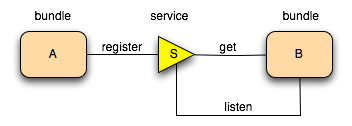
\includegraphics[scale=0.75]{serveLayer.png} 
	\caption{Zależność pomiędzy bundlami i usługami}
\end{figure}
 Możliwe jest oczywiście, żeby dowolna liczba komponentów zarejestrowała ten sam typ usługi lub też pobrała tą samą implementację usługi. Oczywiście zarejestrowane usługi można rozróżniać, każda ma powiązany ze sobą zestaw właściwości(properties), które mogą służyć do specyfikacji. Cała warstwa usług jest dynamiczna, paczki mogą dodawać, usuwać itd. usługi bez konieczności restartu kontenera.  \\
Do tworzenia i definiowana zależności między bundlami OSGi wykorzystuje Blueprint Container. Jest to framework którego celem jest zarządzanie wstrzykiwaniem zależności. Został zaprojektowany żeby radzić sobie z dynamiczną specyfikacją technologii OSGi (możliwość pojawienia się i zniknięcia usługi w dowolnym momencie). Jego specyfikacja pozwala mu też na działania w środowisku innym niż technologii OSGi. W założeniu opiera się on o strukturę plików xml, które definiują jak komponenty są tworzone oraz łączone aby stworzyć działającą aplikację. Sposób działania kontera opiera się o wzorzec Extender. W czasie inicjalizacji paczki (a więc w czasie działania kontenera) Blueprint Container sprawdza czy wszystkie wymagane zależności są spełnione, tworzy wszystkie wymagane obiekty oraz rejestruje usługi. 

Technologia OSGi jest środowiskiem w którym działa budowany system. Każdy komponent systemu jest dostarczany jako osobna paczka OSGi, dzięki czemu może być niezależnie uruchamiany i zarządzany. 

\subsection{Technologia web services}
Technologia web services to system zaprojektowany do wspierania komunikacji między rożnymi komputerami za pomocą sieci.  Podstawowe cechy każdej implementacji tej technologii to:
\begin{itemize}
	\item jest komponentem mogącym być osadzonym w innej aplikacji
	\item komunikacja przy użyciu otwartych protokołów
	\item jest samodzielny i samo-opisujący się
	\item może być zlokalizowany za pomocą UDDI
	\item jest wykorzystywany przez inne aplikacje
\end{itemize}  

Technologia web services jest używana w celu udostępnienia tworzonego systemu jako usługi(Data Endpoints Layer) oraz w celu integracji usług przetwarzania mowy wykorzystujących tą technologię(Services Layer).

Można rozróżnić 2 główne klasy technologii web services :
\begin{itemize}
	\item technologie web services zgodne z architekturą technologii REST
	\item technologie arbitrary web services z których każda może udostępniać dowolny zbiór operacji
\end{itemize}  
\subsubsection{Technologia REST web services}
Usługi z tej grupy \cite{fielding2000} ograniczają swój interfejs do zbioru dobrze znanych i wspieranych przez protokół transportowy operacji takich jak: PUT, GET, POST itd. dla  HTTP. Nacisk jest tutaj skierowany na interakcję z zasobami bezstanowymi. Koncepcja usług technologii REST opiera się na sześciu kluczowych punktach:
\begin{itemize}
	\item model klient-serwer - wprowadza rozdzielenie odpowiedzialności, oznacza to, że na przykład klient nie interesuje się przechowywaniem danych, jest to sprawa wewnętrznej implementacji serwera, a serwer nie interesuje się interfejsem użytkownika co wprowadza prostotę i zwiększa skalowalność
	\item bezstanowość - kontekst aplikacji klienckiej nie jest przechowywany na serwerze pomiędzy zapytaniami, każde nowe zapytanie zawiera wszystkie potrzebne informacje żeby mogło zostać obsłużone
	\item możliwość przechowywania w pamięci podręcznej - aplikacje klienckie mogą przechowywać odpowiedzi w pamięci podręcznej, wymaga to od serwera by odpowiedź była pośrednio lub bezpośrednio zdefiniowana jako możliwa do przechowywania w pamięci podręcznej lub nie, poprawne zarządzanie tą cechą może w sposób znaczny ograniczyć komunikację na linii klient-serwer
	\item warstwowy system - klient nie jest w stanie stwierdzić czy jest bezpośrednio podpięty do usługi czy po drodze znajdują sie inne usługi, takie jak na przykład load-balancer
	\item opcjonalnie wykonanie kodu na żądanie - możliwe jest żeby serwer wykonał kod przesłany przez klienta
	\item jednolity interfejs - upraszcza oraz rozluźnia powiązanie między klientem a serwerem, dzięki temu możliwa jest ich niezależna ewolucja
\end{itemize}   
\subsubsection{Technologia arbitrary web services}
Usługi z tej grupy reprezentują bardziej klasyczne podejście. Do opisania swoich interfejsów mogą (nie jest to wymagane jednak bardzo popularne, co więcej konieczne jeżeli chce się użyć frameworku do generowania kodu) wykorzystywać WSDL. Jest to skrót od Web Service Description Language, formacie bazującym na XML, wykorzystywanym do opisywania jak wywołać daną usługę, jakie parametry wejściowe przyjmuje i jakie struktury danych zwraca. Inne systemy mogą komunikować się z technologią web serwices za pomocą protokołu SOAP. Skrót pochodzi od angielskiej nazwy Simple Object Access Protocol. Dostarcza on standardowy, rozszerzalny, dobrze zdefiniowany fremwork do wymiany wiadomości XML. Wspiera kilka różnych protokołów transportowych takich jak:
 \begin{itemize}
	\item HTTP
	\item SMTP
	\item FTP
	\item RMI/IIOP
\end{itemize}  
\begin{figure}[!h]
	\centering
	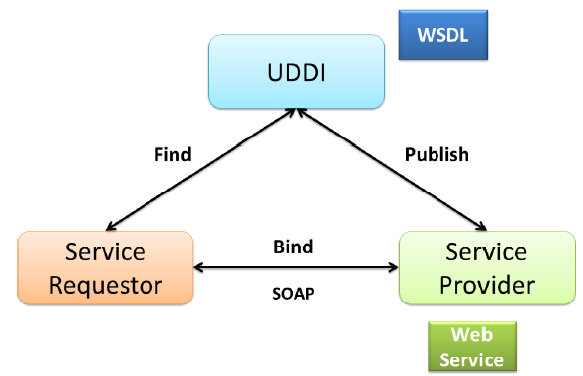
\includegraphics[scale=0.50]{webSerwisyArchitektura.png} 
	\caption{Architektura technologii arbitrary web services}
\end{figure}

\subsection{Apache ServiceMix}
Apache ServiceMix pomaga rozwiązać problem integracji będąc bazującym na standardach, lekkim oraz stosującym paradygmat "luźnego powiązania" narzędziem. Dzięki bazowaniu na standardach w sposób znaczący zmniejsza szanse na uzależnienie się od konkretnego dostawcy oprogramowania, przez stosowanie luźnego powiązania pomiędzy poszczególnymi komponentami zmniejsza złożoność integracji. Jest to otwarta implementacja ESB, zbudowana w oparciu o JBI i wydana na licencji Apache, od wersji 4 ServiceMix wykorzystuje OSGi do uproszczenia podziału aplikacji na komponenty. 	
Architekturę Apache ServiceMix można podzielić na 3 warstwy:
\begin{enumerate}
	\item Warstwa jądra
	\item Warstwa usług
	\item Warstwa aplikacji
\end{enumerate}  
\begin{figure}[!h]
	\centering
	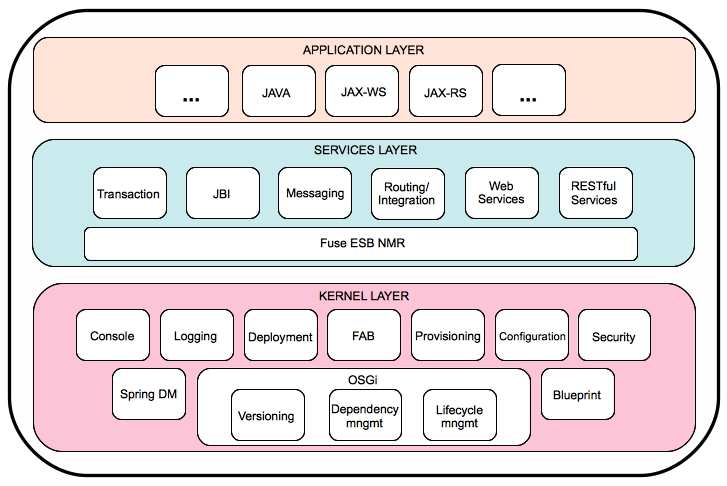
\includegraphics[scale=0.45]{ServiceMixArchitektura.jpg} 
	\caption{Architektura ServiceMix 4}
\end{figure}
Każda z tych warstw ma inne zadania i odpowiada za inne czynności.
\begin{itemize}
	\item Warstwa jądra - bazuje na Apache Karaf czyli implementacji OSGi będącą lekkim kontenerem w którym można osadzić różne komponenty i aplikacje. Warstwa ta współpracuje z warstwą usług w celu stworzenia, skoordynowania, utrzymania i zarządzania logowaniem, bezpieczeństwem oraz transakcjami. Najważniejsze funkcje dostarczane przez tą warstwę to:
	\begin{itemize}
		\item Osadzanie - umożliwia zarówno manualne jak i automatyczne osadzanie bibliotek
		\item Kontener OSGi - ServiceMix 4 wspiera 2 różne kontenery OSGi a mianowicie Eclipse Equinox i Apache Felix
		\item Wstrzykiwanie zależnośći - wykorzystuje 2 różne frameworki:
			\begin{itemize}
				\item Blueprint
				\item Spring DI
			\end{itemize}   
		\item Automatyczna konfiguracja - dokonując zmian w pliku z właściwościami można dokonać zmian "w locie", bez restartowania serwera
		\item Bezpieczeństwo - framework odpowiadający za bezpieczeństwo bazuje na JAAS, dostarcza kilka różnych, odizolowanych poziomów:
			\begin{itemize}
				\item kontenera OSGi
				\item wbudowanej instancji usługi wiadomości
				\item osadzonych instancji usług routingu i integracji
			\end{itemize} 
		\item Logowanie - dynamiczne logowanie wspierające różne interfejsy takie jak: JCL, SLF4J, Avalon, łatwo konfigurowalne poprzez pliki z właściwościami
		\item Konsola - umożliwia zarządzanie i pełną kontrolę nad cała aplikacją
	\end{itemize}  
	\item Warstwa usług - 	składa się z interfejsów i klas reprezentujących wbudowane usługi. Współpracuje z warstwą aplikacji w celu komunikacji z aplikacjami użytkowników które chcą korzystać z oferowanych usług. Najważniejsze funkcje dostarczane przez tą warstwę to:
	\begin{itemize}
		\item Rutowanie i integracja - bazuje na Apache Camel, umożliwia zdefiniowanie ścieżek i zaimplementowanie biznesowych wzorców w celach integracji a następnie osadzenie jako paczka OSGi
		\item Tworzenie usług webowych - bazuje na Apache CXF, umożliwia, w prosty sposób, tworzenie i osadzanie jako paczka OSGi usług webowych implementujących API JAX-WS 
		\item Tworzenie usług webowych zgodnych ze wzorcem REST - bazuje na Apache CXF, umożliwia w prosty sposób, tworzenie i osadzanie jako paczka OSGi usług zgodnych z REST implementujących API JAX-RS
		\item Tworzenie i osadzanie jednostek i zespołów usług bazujących na JBI
		\item Komunikacje - udostępnia usługę wiadomości w całości zbudowaną na Apache ActiveMQ, umożliwiający tworzenie i osadzanie zarówno klientów jak i nadawców wiadomości JMS
		\item Menadżer transakcji - bazuje na Apache Aries, wystawia interfejs transakcji jako usługę, umożliwia tworzenie i osadzanie zarówno aplikacji bazujących na frameworku JTA jak i na technologii Spring
		\item Znormalizowany ruter wiadomości - jego główną rolą jest przekazywanie wiadomości pomiędzy różnymi aplikacjami osadzonymi w kontenerze OSGi oraz, jeżeli zachodzi taka konieczność, pomiędzy aplikacjami z OSGi a aplikacjami osadzonymi w kontenerze JBI
	\end{itemize}
	\item Warstwa aplikacji - w tym miejscu znajdując się aplikacje użytkownika, ServiceMix 4 dostarcza wielu różnych API(częściowo wymienionych w warstwie usług) za pomocą których aplikacje klienckie mogą łączyć się i korzystać z usług oferowanych przez komponenty działające wewnątrz kontenera
\end{itemize}

\subsection{Apache Camel}
Apache Camel \cite{camel2012} \cite{ibsen2010} to framework używany na szeroką skalę w systemach których celem jest rozwiązywanie problemu integracji, na przykład w ServiceMixie. Najważniejszą funkcjonalnością Apache Camel jest mechanizm routingu. W celu lepszego zrozumienia sposobu działania tego frameworku należy wyjaśnić kilka pojęć:
\begin{itemize}
	\item Punkt końcowy - implementacja wzorca Message Endpoint \cite{hohpe2003}, może odnosić się do adresu lub do usługi znajdującego się pod tym adresem (np. źródło RSS, serwer FTP), pozwala wysyłać i odbierać wiadomości  
	\item Komponent - fabryki punktów końcowych, pozwalają w elegancki sposób tworzyć punkty końcowe preferowanego typu na przykład WS, JMS, RSS itd.
	\item Procesor - konsument lub translator wiadomości, może wykonać logikę biznesową lub też wywołać jakąś usługę
	\item Wiadomość - wiadomość technologii Apache Camel
	\item Ścieżka - trasa jaką pokonuje wiadomość, zaczyna się w punkcie końcowym (producent), następnie przechodzi przez procesory(konsumenci) i opcjonalnie może zostać skierowana do innego punktu końcowego
	\item CamelContext - kontekst technologii Apache Camel, miejsce w którym komponenty, punkty końcowe i procesory są zdefiniowane oraz są utworzone ścieżki z ich wykorzystaniem
\end{itemize}  
Korzystając z wszystkich wymienionych wyżej elementów Camel daje możliwość stworzenia bardzo skomplikowanego systemu złożonego z wielu różnych elementów. Za jego pomocą można łatwo zaimplementować system który pobierze plik graficzny z serwera FTP, skieruje go do usługi OCR, następnie tak otrzymany tekst skieruje do usługi TTS. Różnych scenariuszy może być dużo i wszystkie one są łatwe do implementacji z wykorzystaniem technologi Apache Camel. Umożliwia on dwa różne sposoby definiowania ścieżek, za pomocą pliku XML i za pomocą DSL bazującego na języku Java.
\begin{figure}[!h]
	\centering
	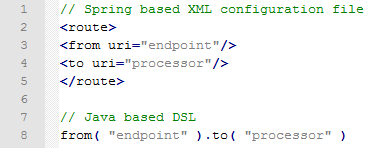
\includegraphics[scale=0.95]{camel.png} 
	\caption{Sposób definiowania ścieżek w technologii Apache Camel}
\end{figure}

W platformie SpeechProcessingPlatform technologia Apache Camel używana jest do komunikacji między poszczególnymi komponentami. Technologia ta dostarcza adresację oraz prosty interfejs do MOM.
	
\section{Technologie przetwarzania mowy}		
\subsection{FreeTTS}
FreeTTS \cite{freettssite} jest syntezatorem mowy, dostępnym na licencji opensource, w całości napisanym w języku Java. Bazuje na silniku Flite stworzonym i rozwijanym przez Carnegie Mellon University. Mimo swojej prostoty jego zaletami są duża wydajność, bardzo dobre radzenie sobie z językiem angielskim oraz częściowe wsparcie dla JSAPI 1.0 (jako, że jest to syntezator nie wspiera części specyfikacji odpowiedzialnej za rozpoznawanie mowy). Dzięki temu ostatniemu w łatwy sposób umożliwia integrację z różnymi, wieloplatformowymi aplikacjami działającymi wewnątrz JVM. Przy opisywaniu tego syntezatora istotną kwestią jest fakt, że posiada dość dobrą dokumentację oraz liczne, łatwe do uruchomienia i, co bardzo ważne, działające dema. Standardowo oferuje 3 różne głosy, wszystkie w języku angielskim, umożliwia jednak rozszerzenie liczby głosów poprzez import nowych stworzonych przy pomocy narzędzi takich jak:
\begin{itemize}
	\item FestVox,
	\item MBROLA,
	\item CMU Arctic.
\end{itemize}    

\subsection{Ivona TTS}
IVONA TTS \cite{ivonasite} to wielojęzyczny syntetyzator mowy działający w oparciu o metodę alofoniczną. Autorski algorytm stosowany przez Ivona nazywa się Bright Voices,  powstał i został opisany podczas Blizzard Challenge 2006. W chwili obecnej funkcjonalność Ivona jest dostępna na dwa sposoby:
\begin{itemize}
	\item poprzez Ivona SDK
	\item poprzez Speech Cloud (SaaS)
\end{itemize}
Ivona SDK to podstawowy sposób korzystania z usług tego oprogramowania. Dostępne są wersję na wiele różnych platform takich jak:
\begin{itemize}
	\item Linux
	\item Windows
	\item iOS
	\item Solaris
\end{itemize}
oraz w kilku różnych językach programowania:
\begin{itemize}
	\item C/C++
	\item Java
	\item ObjectiveC
	\item platforma .NET
\end{itemize}
Dostęp do technologii Speech Cloud możliwy jest zarówno za pomocą protokołu SOAP oraz przez technologię REST. W tej chwili niezależnie od używanego API można uzyskać następującą funkcjonalność:
\begin{itemize}
	\item wygenerowanie pliku dźwiękowego z podanego tekstu
	\item pobranie informacji o dostępnych głosach i kodekach
	\item zmodyfikowanie zasad wymowy, w celu poprawienia jakości wymowy niektórych słów
\end{itemize}
Syntezator ten wspiera bardzo dużo języków między innymi:
 \begin{itemize}
	\item polski
	\item angielski
	\item francuski
	\item portugalski
	\item niemiecki
\end{itemize}
Poza wyborem języka istnieje też możliwość wyboru lektora, różnią się oni barwą i siłą głosu, czy też szybkością mówienia. Możliwa jest też dynamiczna zmiana zarówno języka jak i lektora. Kolejną ważną cechą Ivona jest fakt, iż nie ogranicza się ona do jednego kodeka, wspiera następujące formaty:
\begin{itemize}
	\item mp3/22050
	\item ogg/22050
	\item pcm16/22050
	\item alaw/8000
\end{itemize}
 Aby korzystać ze zdalnego API należy posiadać konto w systemie Ivony, jest ono wykorzystywane do pobierania opłat. Co bardzo istotne, Ivona wspiera protokół SSML, umożliwiający klientowi dokładniejsze sterowanie generowanym głosem. 

\subsection{Google Translate}
Google Translate to płatna usługa Google umożliwiająca tłumaczenie tekstu pomiędzy tysiącami dostępnych par języków. Poza tłumaczeniem usługa ta umożliwia również rozpoznanie języka. API udostępniane przez korporację opiera się o architekturę REST, składa się z trzech metod:
\begin{itemize}
	\item translate - tłumaczy tekst z języka źródłowego na docelowy, przykład:
	\lstset{caption={Tłumaczenie słowa hello z angielskiego na polski},label=DescriptiveLabel}
	\begin{lstlisting}
	https://www.googleapis.com/language/translate/v2?key=INSERT-YOUR-KEY&q=hello%20world&source=en&target=pl
	\end{lstlisting}
	\item languages - zwraca listę języków wspieranych przez translator
	\lstset{caption={Przykład pobrania listy dostępnych języków},label=DescriptiveLabel}
	\begin{lstlisting}
	https://www.googleapis.com/language/translate/v2/languages?key=INSERT-YOUR-KEY&target=zh-TW
	\end{lstlisting}
	\item detect - rozpoznaje język tekstu źródłowego
	\lstset{caption={Przykład detekcji języka},label=DescriptiveLabel}
	\begin{lstlisting}
	https://www.googleapis.com/language/translate/v2/detect?key=INSERT-YOUR-KEY&q=google+translate+is+fast
	\end{lstlisting}
\end{itemize}
Parametr key=INSERT-YOUR-KEY służy korporacji do identyfikowania usługobiorcy, na jego podstawie naliczane są opłaty. Jak widać REST w API Google Translate różni się nieznacznie od tradycyjnego pojmowania tej architektury. Zamiast dostarczać dostęp do zasobów, dostarczany jest dostęp do usług, stosując takie podejście uzyskano możliwość wykorzystania jednego URI jako całego API. 

\subsection{OCR Web Service}
OCR Web Service jest to jeden z najpopularniejszych technologii web serwices tego rodzaju. Rozpoznaje aż dwadzieścia osiem języków między innymi:
\begin{itemize}
	\item polski
	\item angielski
	\item niemiecki
	\item francuski
	\item portugalski
\end{itemize}
Przyjmuje różne formaty wejściowe, takie jak: JPEG/JPG, BMP, PCX, GIF, PNG, PDF. Co więcej pozwala na przekonwertowanie rozpoznanego tekstu na aż pięć różnych formatów:
\begin{itemize}
	\item Adobe PDF
	\item MS Word 2003
	\item MS Excel 2003
	\item HTML
	\item RTF
\end{itemize}
Oczywiście istnieje też możliwość otrzymania zwykłego pliku txt. Wymagania tej usługi co do jakości obrazu w pliku otrzymanym na wejściu też nie są duże, zaleca się aby rozdzielczość wynosiła między 200 a 400 dpi. Usługa ta, jako protokół komunikacyjny wykorzystuje SOAP w wersji 1.1 lub 1.2. WSDL potrzebny do wygenerowania szkieletu kodu można pobrać ze strony projektu. Jedną z niewielu wad tej usługi jest to, że podobnie jak Google Translate jest płatna. 						% aims of the project

% this file is called up by thesis.tex
% content in this file will be fed into the main document

%: ----------------------- name of chapter  -------------------------
\chapter{Weryfikacja rozwiązania} % top level followed by section, subsection


%: ----------------------- paths to graphics ------------------------

% change according to folder and file names
\ifpdf
    \graphicspath{{4/figures/PNG/}{4/figures/PDF/}{4/figures/}}
\else
    \graphicspath{{4/figures/EPS/}{4/figures/}}
\fi

%: ----------------------- contents from here ------------------------

Rozdział ten jest podzielony na trzy części. Część pierwsza opisuje jak wybrany sposób integracji oraz powstały w ten sposób prototypowy system wpływa na łatwość tworzenia i efektywność aplikacji przetwarzających mowę. Proponowane przykładowe aplikacje to:
\begin{itemize}
	\item Automatyczne dyktando
	\item Lektor RSS
	\item Lektor SMS
	\item Konwerter plików graficznych do tekstowych
\end{itemize}
Każdej z proponowanych aplikacji poświęcono osobny podpodrozdział, w którym jest zdefiniowany przypadek użycia, przedstawione są wymagania funkcjonalne i niefunkcjonalne oraz przedstawiona jest weryfikacja podejścia. Część druga tego rozdziału opisuje testy (i ich wyniki) którym została poddana prototypowa implementacja systemu. Ostatnia część wynikające z części poprzednich.

\section{Weryfikacja funkcjonalności}
\subsection{Automatyczne dyktando}
Jest to aplikacja webowa umożliwiająca użytkownikowi ćwiczenie pisowni w różnych językach. Zasada działania jest bardzo prosta, użytkownik ładuje plik tekstowy lub graficzny na serwer oraz wybiera język docelowy, następnie zostaje przekierowany na stronę zawierającą formularz do pisania tekstu oraz odtwarzacz. Użytkownik słucha tekstu i zapisuje w polu tekstowym transkrypcję. W momencie w którym zatwierdzi formularz zostaje on przesłany na serwer i porównany z oryginalnym plikiem wejściowym, w efekcie użytkownik otrzymuje informację o ilości popełnionych błędów oraz o wyrazach które źle zapisał. 
\subsubsection{Przypadek użycia}
\begin{figure}[!h]
	\centering
	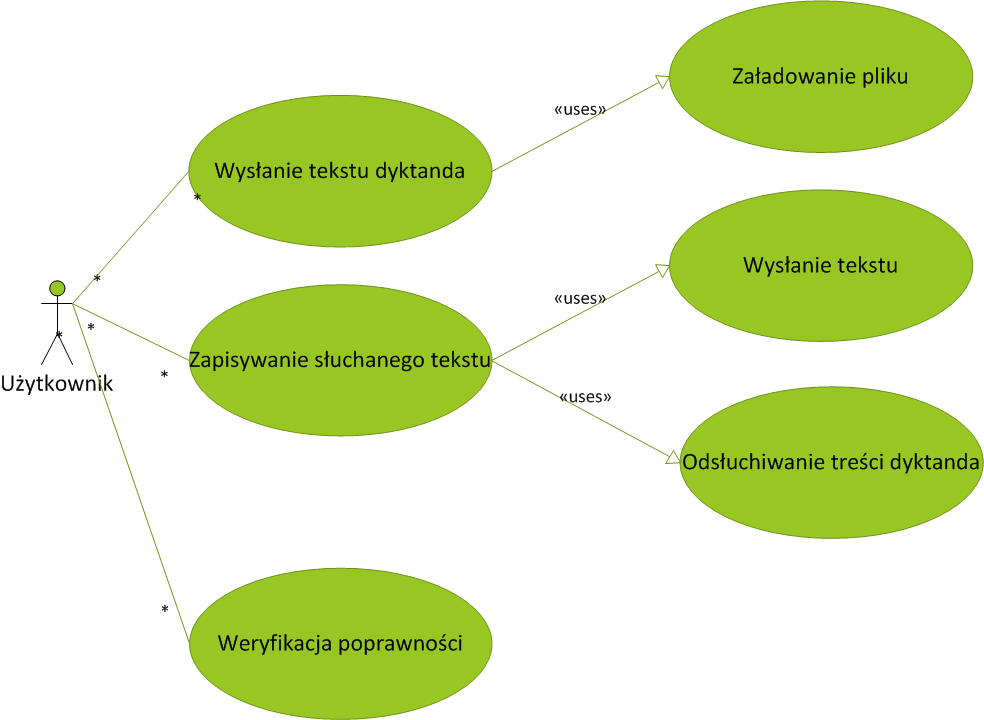
\includegraphics[scale=0.45]{useCaseDictando.png} 
	\caption{Przypadek użycia - Automatyczne dyktando }
\end{figure}


\subsubsection{Wymagania funkcjonalne}
\begin{enumerate}
	\item Obsługiwanie wielu języków
	\item Możliwość podania tekstu źródłowego
		\begin{enumerate}
			\item jako plik graficzny
			\item jako plik tekstowy, wysyłany na serwer
		\end{enumerate}
	\item Umożliwienie użytkownikowi odsłuchania wysłanego tekstu w wybranym przez niego języku
	\item Umożliwienie użytkownikowi wprowadzania tekstu jednocześnie z odsłuchiwaniem
	\item Wygenerowanie i wyświetlenie raportu o ilości błędów popełnionych przez użytkownika
\end{enumerate}

\subsubsection{Wymagania niefunkcjonalne}
\begin{enumerate}
	\item Bezpieczeństwo - użytkownik i tylko on powinien móc widzieć swoje wyniki
	\item Wydajność - dyktowanie tekstu powinno przebiegać płynnie, opóźnienie może występować tylko przed rozpoczęciem, od 0 do 60 sekund, przerwy w czasie dyktowania tekstu są niedopuszczalne
	\item Niezawodność - użytkownik powinien zawsze otrzymać wynik który jest poprawny, tzn. pokazuje dokładną ilość błędów popełnionych przez użytkownika
\end{enumerate}

\subsubsection{Weryfikacja podejścia}
Jak widać w powyższym podrozdziale wymagania stawiane przed aplikacją są precyzyjne i klarowne. Zastosowane podejście integracyjne sprawia, że stworzenie aplikacji spełniającej wymagania staje się proste. Zapewnienie obsługi wielu języków nie wymaga praktycznie żadnego nakładu pracy ze strony programisty aplikacji klienckiej. Jak zostało to opisane w rozdziale drugim, przy zastosowanym podejściu wystarczy wygenerować i przesłać plik xml z informacją dotyczącą języka docelowego, działa to niezależnie od języka w którym jest tekst wejściowy (pod warunkiem, że w pliku konfiguracyjnym ustawi się tag odpowiedzialny za serwis rozpoznający język). Podobnie przesłanie pliku graficznego, również wymaga tylko umieszczenia odpowiedniego tagu w pliku xml celem wywolania serwisu OCR. Jak łatwo zauważyć wygenerowanie i przesłanie pliku xml nie jest dużym wyzwaniem programistycznym.Widać to szczególnie gdyby porównać to z implementacją bez wykorzystania systemu opartego o rozwiązanie opisane w tej pracy. Musiałaby ona łączyć się z kilkoma zewnętrznymi serwisami, z których każdy prawdopodobnie miałby inny interfejs, konwertować różne formaty plików, obsługiwać błędy itd. Jak widać, w tym przypadku, zastosowane podejście w sposób znaczący pozytywnie wpływa na łatwość i szybkość implementacji aplikacji klienckiej, co więcej sprawia ono, że w przyszłości aplikacja może zostać rozbudowana lub też łatwo przeniesiona na inne platformy np. telefony. \\

\subsection{Lektor SMS}
Jest to aplikacja przeznaczona dla systemu operacyjnego Android. Jak nazwa wskazuje jej funkcjonalność pozwala odczytywać na głos wiadomości tekstowe. Może okazać się bardzo przydatna w czasie jazdy samochodem, wiadomo, że używanie telefonu komórkowego jest zabronione z powodu bezpieczeństwa, tym bardziej, używanie rąk i skupianie wzroku na odczytywanej wiadomości tekstowej jeszcze w większym stopniu niż rozmowa przez telefon prowadzi do odwrócenia uwagi kierowcy od sytuacji na drodze.
Zasada działania tej aplikacji jest bardzo prosta, mianowicie po włączenie przechwytuje ona każde zdarzenie oznaczające otrzymanie wiadomości tekstowej, pobiera jej treść i zamienia ją na dzwięk w dowolnym, wybranym przez użytkownika języku. Co warte zauważenia aplikacja ta ma dwa różne sposoby generowania mowy:
\begin{itemize}
	\item korzystając z usług udostępnianych przez przykładową implementację systemu integrującego usługi przetwarzania mowy
	\item korzystając z wbudowengo w system Android TTS'a
\end{itemize} 
Dzięki wykorzystaniu obu rozwiązań mamy możliwość bezpośredniego porównania. Wybór sposobu generowania dzwięku zależy od dostępności połączenia z internetem, jeżeli takie istnieje to aplikacja korzysta z zewnętrznego systemu, w przeciwnym razie wykorzystuje wbudowany TTS. Oczywiście użytkownik ma możliwość ustawienia dla których numerów aplikacja będzie działać.
\newpage
\subsubsection{Przypadek użycia}
\begin{figure}[!h]
	\centering
	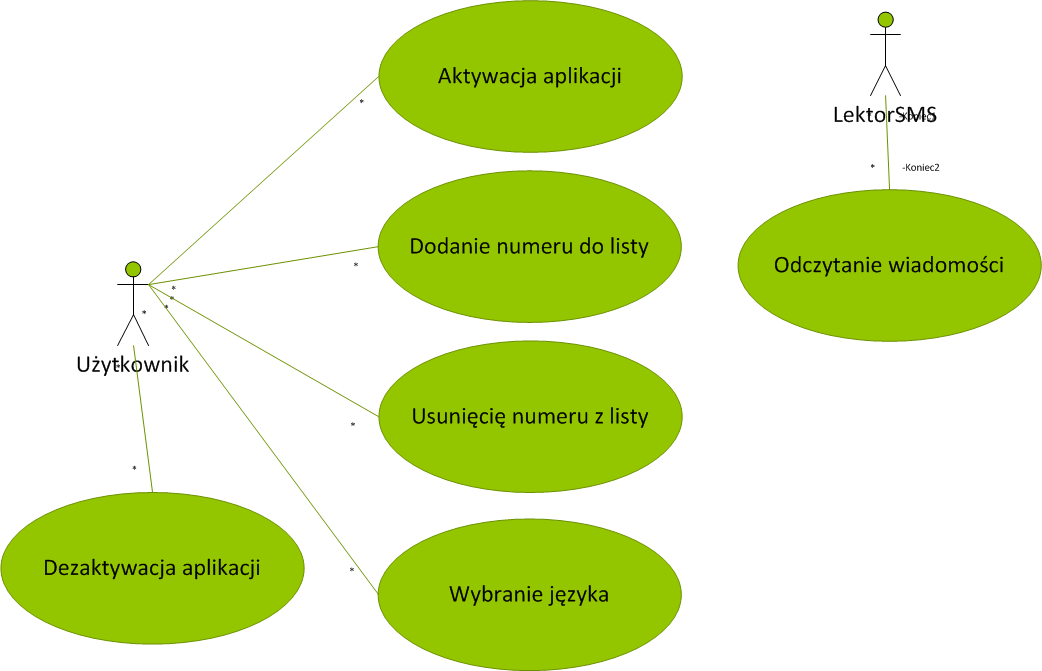
\includegraphics[scale=0.45]{useCaseLektorSMS.png} 
	\caption{Przypadek użycia - LektorRSS}
\end{figure}

\subsubsection{Wymagania funkcjonalne}
\begin{enumerate}
	\item Możliwość aktywacji i dezaktywacji aplikacji
	\item Możliwość ustawienia języka w którym będzie odczytywana treść wiadomości
	\item Możliwość filtrowania obsługiwanych wiadomości SMS po numerach nadawców 
	\item Obsługiwanie więcej niż jednego języka wiadomości
	\item Automatyczne odczytywanie otrzymanych wiadomości
\end{enumerate}
\subsubsection{Wymagania niefunkcjonalne}
\begin{enumerate}
	\item Dostęp do apikacji musi być chroniony hasłem
	\item Użyteczność - poprawne działanie na dowolnym urządzeniu z systemem Android z dostępem do siecii lub z systemem w wersji co najmniej 1.6
\end{enumerate}

\subsubsection{Weryfikacja podejścia}
Wykorzystanie sposobu integracji systemów przetwarzania mowy rozważanego w tej pracy pozwala na bardzo łatwą implementację aplikacji spełniającej wszystkie stawiane przed nią wymagania. Co więcej pozwala ona na łatwą rozbudowę. Można na przykład dodać funkcjonalność polegającą na tłumaczenie wiadomości na konkretny język docelowy, co w implementacji bez wykorzystania systemu byłoby dużo trudniejsze i wymagało przesłania większej ilości danych co ponosi za sobą koszty(szczególnie jeżeli telefon działa w roamingu). Z drugiej strony system Android daje dostęp do wbudowanej usługi TTS. Jest ona dość dobrej jakości, również obsługuje kilka języków, nie wymaga dostępu do internetu co jest jej dużym plusem. Implemetancja aplikacji z jej wykorzystaniem również jest prostym zadaniem. Na podstawie wszystkich argumentów można dojść do wniosku, że w tym przypadku nie ma potrzeby korzystania z koncepcyjnego systemu. Dlatego też, w tym konkretnym przypadku, ciężko ocenić które rozwiązanie jest lepsze. Wszystko zależy od tego czy ważniejsza jest jakość wygenerowanego dźwięku, możliwość dodania dodatkowych funkcji czy szybkość działania i nie obciążanie połączenia internetowego.

\subsection{Lektor RSS}
Jest to aplikacje webowa której zadaniem jest odczytywanie wiadomości RSS ze źródeł podanych przez użytkownika, może on podać źródło przez specjalny formularz, załadować plik tekstowy zawierający adresy źródeł. Niezależnie od użytej metody można podać język wiadomości lub też użyć serwisu rozpoznającego. Możliwe jest również przetłumaczenie wiadomości na język podany przez użytkownika i dopiero wtedy przeczytanie jej przez odpowiedniego lektora. Użytkownik ma również możliwość ustawienia co jaki czas ma następować sprawdzanie źródła celem znalezienia nowych wiadomości.	 
\newpage
\subsubsection{Przypadek użycia}
\begin{figure}[!h]
	\centering
	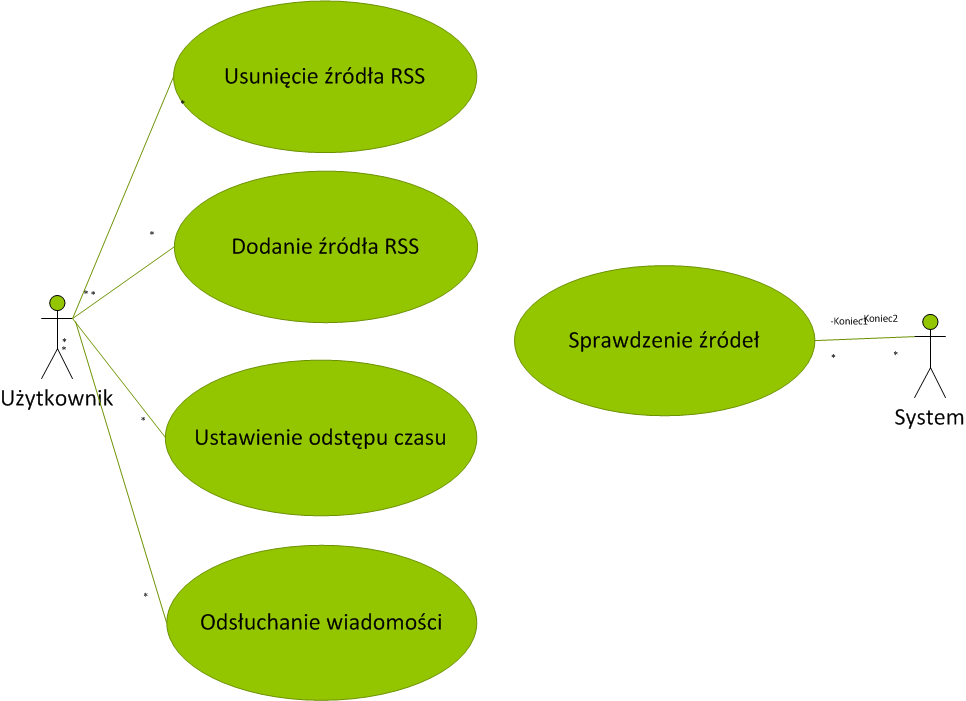
\includegraphics[scale=0.45]{useCaseRSS.png} 
	\caption{Przypadek użycia - LektorRSS}
\end{figure}

\subsubsection{Wymagania funkcjonalne}
\begin{enumerate}
	\item Możliwość dodania źródła RSS
	\item Możliwość usunięcia źródła RSS
	\item Obsługiwanie więcej niż jednego języka wiadomości
	\item Automatyczne sprawdzanie czy któreś ze źródeł nie zawiera nowej wiadomości
	\item Możliwość ustawienia odstępów czasowych pomiędzy sprawdzaniem przez system źródeł
	\item Automatyczne Odczytanie użytkownikowi nowych wiadomości (w przypadku istnienia) 
\end{enumerate}  
\subsubsection{Wymagania niefunkcjonalne}
\begin{enumerate}
	\item Niezawodność - system nie może pominąć żadnej wiadomości z listy źródeł zdefiniowanej przez użytkownika
	\item Szybkość - różnica czasu pomiędzy udostępnieniem nowej wiadomości w którymś ze źródeł a otrzymaniem jej przez użytkownika nie może przekraczać czasu pomiędzy sprawdzeniami w poszukiwaniu uaktualnień (czas ten ustawia użytkownik)
	\item Możliwość personalizacji - użytkownik powinien móc dodać dowolną ilość różnych źródeł, system powinien zapewnić ich niepowtarzalność(usuwać duplikaty)
\end{enumerate}

\subsubsection{Weryfikacja podejścia}
Tak jak w sekcji opisującej aplikację Automatyczne Dyktando wymagania przedstawione powyżej są jasne i klarowne. Po raz kolejny zastosowane podejście integracyjne sprawia, że napisanie aplikacji klienckiej, spełniającej wymagania przed nią stawiane jest proste. Dzięki użyciu ESB i oferowanych przez niego punktów końcowych jest możliwe przerzucenie konieczności pobierania wiadomości ze źródeł RSS na stronę systemu. Podobnie jak w przypadku aplikacji opisanej wyżej zarówno rozpoznawanie języka, tłumaczenie czy generowanie mowy w odpowiednim języku nie stanowi dla programisty, autora aplikacji klienckiej, żadnego problemu, wystarczającym jest wygenerowanie pliku xml zawierającego odpowiednie instrukcje. Implementacja podobnej, równie rozbudowanej aplikacji, bez wykorzystania systemu integrującego serwisy odpowiadające za przetwarzanie mowy, byłaby trudniejsza oraz wymagałaby poświęcenia większej ilości czasu. Poza problemami podobnymi do tych jakie były opisane w przypadku Aumatycznego Dyktanda dochodzi jeszcze sprawa pobierania RSS'ów, ich parsowania itd. Pozostałe wymagania, takie jak bezpieczeństwo czy też konieczność przechowywania danych w bazie danych muszą być zaspokojone w ten sam sposób niezależnie od wykorzystania systemu. \\
W przypadku tej aplikacji również klarownym jest fakt, że zastosowane podejście bardzo upraszcza implementację.

\section{Weryfikacja wydajności}
W części tej opisane są wyniki testów jak i testy którym został poddany prototyp platformy oraz ich porównanie z wynikami testów przeprowadzonych bezpośrednio na integrowanych serwisach.
\subsection{Serwis TTS}
Test dla serwisu TTS polegał na syntezie tekstu  w języku angielskim, zamieszczonego na rysunku\ref{fig:ttsExample}.
\begin{figure}[!h]
\centering
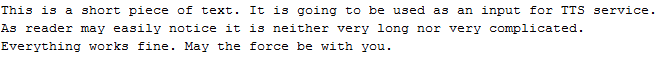
\includegraphics[scale=0.9]{textExample.png}
\caption{Przykładowy tekst dla serwisu TTS}\label{fig:ttsExample}
\end{figure}
Ponieważ w obu przypadkach wykorzystano ten sam tekst jakość odczytu była taka sama. Jedyna różnica występuje w czasie działania. Próbę powtorzono dziesięciokrotnie, wyniki można zaobserwować w tabeli \ref{tab:TTS}. Należy zaznaczyć, że ''Web service'' oznacza bezpośrednie wywołanie serwisu TTS, a ''Prototyp'' wywołanie usługi poprzez przykładową implementację platformy integracyjnej.
\begin{center}
	\begin{table}[h]
	\label{tab:TTS}
	\caption{Test TTS}
	\centering
	\begin{tabular}{| l | l | l |}	
		\hline
		\textbf{Numer testu} & \textbf{Web service [ms]} & \textbf{Prototyp [ms]} \\ \hline
		1 & 1332 & 1476\\ \hline
		2 & 1376 & 1493\\ \hline
		3 & 1241 & 1387\\ \hline
		4 & 1250 & 1315\\ \hline
		5 & 1236 & 1489\\ \hline
		6 & 1225 & 1424\\ \hline
		7 & 1288 & 1398\\ \hline
		8 & 1234 & 1503\\ \hline
		9 & 1184 & 1131\\ \hline
		10 & 1230 & 1543\\ \hline
		\textbf{Średnia/Odchylenie standardowe} & 1256.6/145.182 & 1415.9/84.14\\ 
		\hline
	\end{tabular}
	\end{table}
\end{center}
Jak łatwo można zaobserwować koszt czasowy użycia prototypowego systemu nie jest duży. Co więcej jest on stabilny, nie odnotowano wystąpień dużych odchyleń. 

\subsection{Serwis Translacji}
Test dla serwisu translacji polegał na tłumaczeniu tekstu z języka polskiego na język angielski. Tekst który posłuzył nam w tym teście został zamieszczony na rysunku \ref{fig:translatorExample}.
\begin{figure}[!h]
\centering
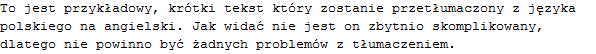
\includegraphics[scale=0.9]{translatorExample.png}
\caption{Przykładowy tekst dla serwisu translacji}\label{fig:translatorExample}
\end{figure}
Ponieważ użyto tego samego serwisu tłumaczącego jego efekt za każdym razem był taki sam. Rysunek \ref{fig:translatorResult} przedstawia tekst wynikowy, efekt można uznać za zadowalający acz nie bezbłędny. 
\begin{figure}[!h]
\centering
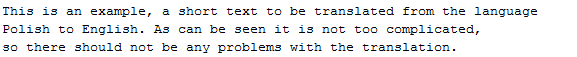
\includegraphics[scale=0.9]{translatorResult.png}
\caption{Wynik translacji}\label{fig:translatorResult}
\end{figure}

Próbę powtórzono dziesięciokrotnie, wyniki można zaobserwować w tabeli \ref{tab:translacja}. Należy zaznaczyć, że ''Web service'' oznacza bezpośrednie wywołanie serwisu translacji, a ''Prototyp'' wywołanie usługi poprzez przykładową implementację platformy integracyjnej.
\begin{center}
	\begin{table}[h]
	\label{tab:translacja}
	\caption{Test Translacji}
	\centering
	\begin{tabular}{| l | l | l |}	
		\hline
		\textbf{Numer testu} & \textbf{Web service [ms]} & \textbf{Prototyp [ms]} \\ \hline
		1 & 618 & 560\\ \hline
		2 & 477 & 801\\ \hline
		3 & 433 & 546\\ \hline
		4 & 407 & 593\\ \hline
		5 & 390 & 550\\ \hline
		6 & 437 & 774\\ \hline
		7 & 645 & 683\\ \hline
		8 & 430 & 501\\ \hline
		9 & 394 & 578\\ \hline
		10 & 410 & 618\\ \hline
		\textbf{Średnia/Odchylenie standardowe} & 464.1/38.01645 & 620.4/41.7235\\ 
		\hline
	\end{tabular}
	\end{table}
\end{center}
Koszt czasowy wykorzystania prototypu nie jest duży, co więcej nie odnotowano wystąpień dużych odchyleń, co świadczy o stabilności.

\subsection{Serwis OCR}
Test dla serwisu OCR polegał na rozpoznawaniu tekstu znajdującego się na obrazku w formie jpg, obrazek jest przedstawiony na rysunku \ref{fig:OCRExample}. 
\begin{figure}[!h]
\centering
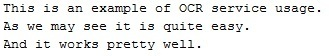
\includegraphics[scale=0.9]{OCRExample.jpg}
\caption{Plik wejściowy dla serwisu OCR}\label{fig:OCRExample}
\end{figure}
Ponieważ użyto tego samego serwisu OCR jego efekt za każdym razem był taki sam. Rysunek \ref{fig:OCRResult} przedstawia tekst wynikowy, efekt można uznać za bezbłędny acz należy wziąć pod uwagę prostotę tego przykładu.
\begin{figure}[!h]
\centering
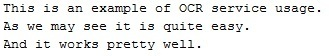
\includegraphics[scale=0.9]{OCRExample.jpg}
\caption{Wynik działania serwisu OCR}\label{fig:OCRResult}
\end{figure}
Próbę powtórzono dziesięciokrotnie, wyniki można zaosberwować w tabeli \ref{fig:ocr}. Należy zaznaczyć, że ''Web service'' oznacza bezpośrednie wywołanie serwisu OCR, a ''Prototyp'' wywołanie usługi poprzez przykładową implementację platformy integracyjnej.
\begin{center}
	\begin{table}[h]
	\label{fig:ocr}
	\caption{Test OCR}
	\centering
	\begin{tabular}{| l | l | l |}	
		\hline
		\textbf{Numer testu} & \textbf{Web service [ms]} & \textbf{Prototyp [ms]} \\ \hline
		1 & 2961 & 3712\\ \hline
		2 & 3509 & 5486\\ \hline
		3 & 4427 & 4135\\ \hline
		4 & 5258 & 4444\\ \hline
		5 & 3929 & 4052\\ \hline
		6 & 3641 & 3084\\ \hline
		7 & 4012 & 4550\\ \hline
		8 & 4321 & 3632\\ \hline
		9 & 5363 & 5381\\ \hline
		10 & 3589 & 3764\\ \hline
		\textbf{Średnia/Odchylenie standardowe} & 4101/472.1354 & 4224/457.2335\\ 
		\hline
	\end{tabular}
	\end{table}
\end{center}
Koszt czasowy wykorzystania protorypu nie jest duży, co więcej nie odnotowano wystąpień dużych odchyleń, co świadczy o stabilności. 

\subsection{Test złożony}
Celem tego testu było wypróbowanie bardziej złożonego scenariusza jakim jest wysłanie do prototypowej implementacji systemu pliku graficznego wraz z plikiem konfiguracyjnym xml przedstawionym na rysunku \ref{fig:xmlConf}.
\begin{figure}[!h]
\centering
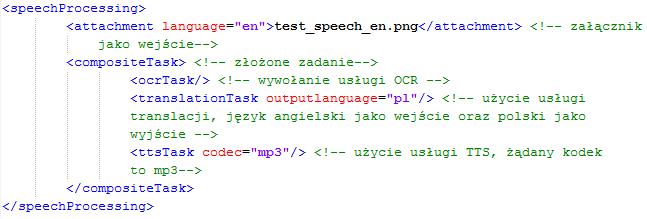
\includegraphics[scale=0.9]{xmlConf.png}
\caption{Plik konfiguracyjny xml}\label{fig:xmlConf}
\end{figure}
W jego wyniku otrzymano plik dźwiękowy w formacie mp3, zawierający odczyt tekstu będącego tłumaczeniem tekstu znajdującego się na obrazku \ref{fig:OCRExample} wysłanym na wejście. Gdyby zapisać zdania czytane przez lektora wyglądałyby one następująco: ''To jest przykład użycia OCR usług. Jak możemy zobaczyć, jest to dość proste. I to działa całkiem dobrze.''. Nie stwierdzono żadnych niewyraźnie przeczytanych wyrazów, ani innych nieprawidłowości. Tłumaczenie również jest całkiem poprawne. Test powtórzono dziesięciokrotnie, wyniki są zaprezentowane w tabeli \ref{tab:bigTest}. Należy zaznaczyć, że ''Web service'' oznacza bezpośrednie wywołanie serwisów, a ''Prototyp'' wywołanie usługi poprzez przykładową implementację platformy integracyjnej.
\begin{center}
	\begin{table}[t]
	\label{tab:bigTest}
	\caption{Test złożony}
	\centering
	\begin{tabular}{| l | l | l |}	
		\hline
		\textbf{Numer testu} & \textbf{Web services [ms]} & \textbf{Prototyp [ms]} \\ \hline
		1 & 4911 & 5552\\ \hline
		2 & 5362 & 7264\\ \hline
		3 & 6101 & 6308\\ \hline
		4 & 6915 & 6268\\ \hline
		5 & 5555 & 5626\\ \hline
		6 & 5303 & 5878\\ \hline
		7 & 5945 & 7238\\ \hline
		8 & 5985 & 6424\\ \hline
		9 & 6941 & 5685\\ \hline
		10 & 5229 & 5234\\ \hline
		\textbf{Średnia/Odchylenie standardowe} & 5824.7/843.4343 & 6147.7/823.7793\\ 
		\hline
	\end{tabular}
	\end{table}
\end{center}
\newpage
Jako czas potrzebny na wykonanie scenariusza w przypadku bezpośredniego wywołania serwisów wzięto sumę czasów potrzebnych do wywołania każdego z osobna. W przypadku wykorzystania prototypowego systemu czas wykonania usługi nie jest znacząco większy niż przy bespośrednim wywołaniu serwisów. Co więcej jest on mniejszy niż gdyby zsumować czas potrzebny na wywołanie każdej z usług osobno za pomocą platformy. Prawdopodobnie wynika to z faktu, że przy wywołaniu złożonego scenariusza mamy tylko jedno zapytanie na drodze klient - platforma, zamiast trzech które byłyby potrzebne do wywołania każdej usługi osobno.  

\section{Wnioski}
Jak widać zastosowanie prototypowej  platformy wprowadza pewien narzut czasowy, nie jest on jednak duży. W zamian klient takiego serwisu integracyjnego otrzymuje znacznie prostszy interfejs, który mimo swojej prostoty daje duże możliwości. Co więcej klient nie musi martwić się o potencjalne błędy, konwersje między formatami, niedostępność któregoś z serwisów itd. Podsumowując, zastosowanie takiej platformy jest uzasadnione, jest ona funkcjonalna, nie wprowadza opóźnień oraz posiada szeroki zakres usług. 
Jak widać 
% ---------------------------------------------------------------------------
%: ----------------------- end of thesis sub-document ------------------------
% ---------------------------------------------------------------------------

						
	
%% this file is called up by thesis.tex
% content in this file will be fed into the main document

%: ----------------------- name of chapter  -------------------------
\chapter{Implementacja projektów} % top level followed by section, subsection


%: ----------------------- paths to graphics ------------------------

% change according to folder and file names
\ifpdf
    \graphicspath{{5/figures/PNG/}{5/figures/PDF/}{5/figures/}}
\else
    \graphicspath{{5/figures/EPS/}{5/figures/}}
\fi

%: ----------------------- contents from here ------------------------


W rozdziale trzecim zostały przedstawione wymagania funkcjonalne i niefunkcjonalne stawiane przed przykładowymi aplikacjami mogącymi korzystać z systemu którego implementacja była celem tej pracy. Niniejszy rozdział opisuje sposób implementacji tych aplikacji.
\section{Automatyczne dyktando}
Automatyczne dyktando, jak już zostało opisane w rozdziale trzecim, jest to prosty serwis internetowy umożliwiający użytkownikowi ćwiczenie ortografii. Jak większość współczesnych aplikacji internetowych ma budowę warstwową, składa się z 3 warstw:
\begin{itemize}
	\item prezentacji,
	\item logiki biznesowej,
	\item komunikacji z serwisem UniversalSynthesizer.
\end{itemize}
\begin{figure}[!h]
	\centering
	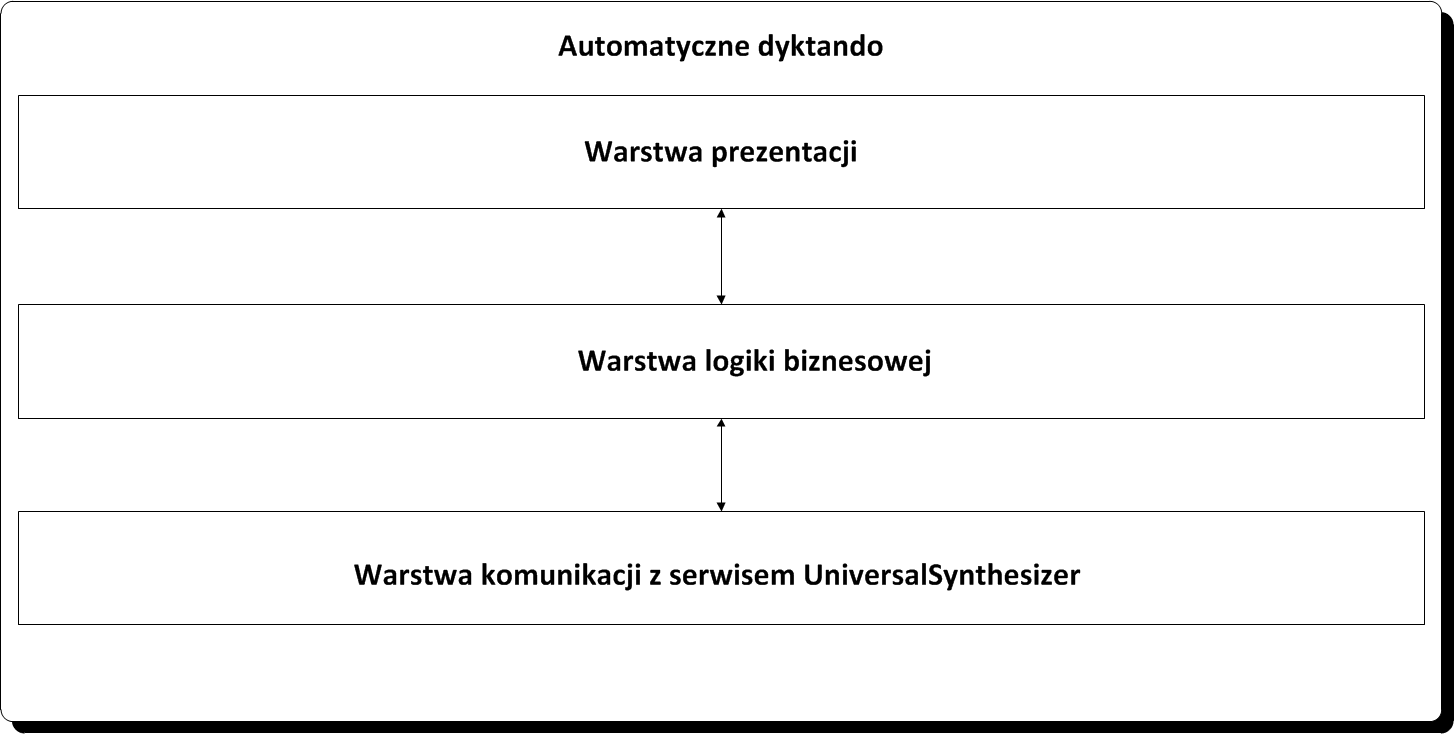
\includegraphics[scale=0.45]{automatyczneDyktandoArchitektura.png} 
	\caption{Automatyczne Dyktanto Architektura}
\end{figure}
Do stworzenia szkieletu tej aplikacji wykorzystano framework Spring MVC, do tworzenia widoków framework Freemarker a do komunikacji z serwisem UniversalSyntesizer bibliotekę jersey-client będącą implementacją JAX-RS. 
\newpage
\subsection{Warstwa prezentacji}
W skład warstwy prezentacji wchodzą trzy strony:
\begin{itemize}
	\item strona główna - umożliwiająca podanie tekstu lub też załadowanie pliku tekstowego, który posłuży jako treść dyktanda
	\item strona z odtwarzaczem - umożliwiająca odsłuchanie tekstu i napisanie jego transkrypcji
	\item strona z wynikami - pokazująca ilość błedów popełnionych przez użytkownika
\end{itemize}
Dodatkowo z każdej z wyżej wymienionych stron istnieje możliwość powrotu do głównej. \\
Jak już wspomniano wyżej, do przygotowania widoków użyto szablonów Freemarker'owych, po jednym na każdą z wymienionych stron, plus jeden dodatkowy, przeznaczonydo ładowania plików na serwer. Dzięki wykorzystaniu Spring MVC i wsparciu które zapewnia implementacja kontrolerów i możliwego przepływu sterowania była sprawą trywialną. s
\subsection{Warstwa logiki biznesowej}

\subsection{Warstwa komunikacji z serwisem UniversalSynthesizer}

\section{LektorsRSS}

\section{LektorSMS}




% ---------------------------------------------------------------------------
%: ----------------------- end of thesis sub-document ------------------------
% ---------------------------------------------------------------------------


% this file is called up by thesis.tex
% content in this file will be fed into the main document

%: ----------------------- name of chapter  -------------------------
\chapter{Projekt i implementacja systemu SpeechProcessingPlatform} % top level followed by section, subsection


%: ----------------------- paths to graphics ------------------------

% change according to folder and file names
\ifpdf
    \graphicspath{{6/figures/PNG/}{6/figures/PDF/}{6/figures/}}
\else
    \graphicspath{{6/figures/EPS/}{6/figures/}}
\fi

%: ----------------------- contents from here ------------------------

Rozdział ten opisuje architekturę, projekt i implementację przykładowej platformy integracyjnej SpeechProcessingPlatform, która umożliwi weryfikację proponowanego podejścia. Platforma ta jest projektowana z myślą o architekturze opartej na technologii ESB, którą autorzy uznali za najlepiej nadającą się do realizacji systemów integracyjnych. Rozdział ten zawiera opis najważniejszych części systemu, zależności między nimi oraz formatu danych wykorzystywanego w komunikacji.

\section{Architektura}

Rysunek \ref{fig:layered_architecture} przedstawia architekturę systemu SpeechProcessingPlatform. Jest ona podzielona na 3 warstwy:

\begin{itemize}
	\item Data Endpoints Layer
	\item Routing Layer
	\item Services Layer
\end{itemize}

\begin{figure}[!h]
	\centering
	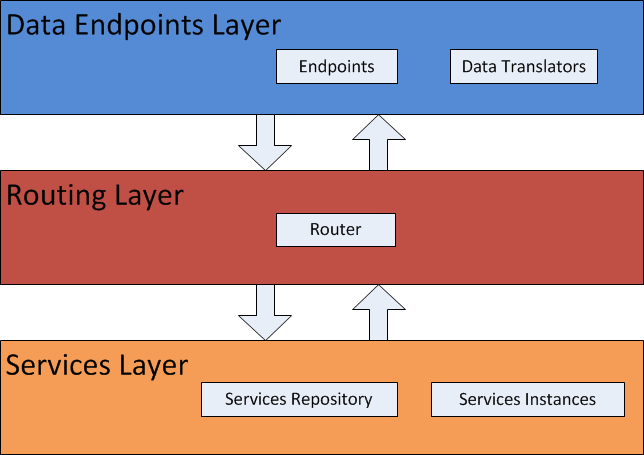
\includegraphics[scale=0.7]{layered_architecture.png}
	\caption{Architektura systemu SpeechProcessingPlatform}\label{fig:layered_architecture}
\end{figure}

Podejście warstwowe ułatwia dekompozycję systemu na niezależne komponenty, które odpowiadają za dobrze zdefiniowany fragment wymaganej funkcjonalności. 
% tu mozna cos dodac jak cos

Warstwa \textit{Data Endpoints Layer} odpowiada za udostępnianie interfejsów dla aplikacji klienckich oraz za transformacje danych do wspólnego formatu. Głównymi elementami tej warstwy są punkty końcowe i translatory danych. Punkty końcowe wystawiają interfejsy umożliwiające dostęp do platformy przy użyciu różnych technologii takich jak REST, FTP, SOAP czy RSS. Zadaniem translatorów jest ujednolicenie danych do postaci używanej w kolejnych warstwach. Dzięki temu komponenty z warstw niższych mają uproszczoną implementację ponieważ skupiają się na obsłudze tylko jednego, dobrze zdefiniowanego formatu. 

Warstwa \textit{Routing Layer} odpowiada za routowanie zadań przetwarzania od punktów końcowych do odpowiednich serwisów, a także za przesyłanie wyników z powrotem do punktów końcowych. Zadania mogą być jedno etapowe jak np. \textit{przetłumacz ten tekst z języka polskiego na język angielski} albo dwu lub więcej etapowe jak np. \textit{rozpoznaj tekst na tym zdjęciu, jeżeli trzeba przetłumacz na język angielski i na jego podstawie wygeneruj dźwięk}.

Głównym elementami ostatniej warstwy, \textit{Services Layer}, jest repozytorium serwisów oraz konkretne ich instancje. Główne zadanie repozytorium to wyszukiwanie i zwracanie odpowiednich instancji w odpowiedzi na żądania warstwy routującej. Najważniejszą cechą wyróżniającą poszczególne serwisy jest typ przetwarzania mowy jaki dostarczają. Ze względu na to kryterium zostały one podzielone na 5 grup, a każda z nich posiada dodatkowe cechy, które także mają wpływ na wynik wyszukiwania:

\begin{itemize}
	\item OCR
	\begin{itemize}
		\item wejście - plik graficzny, parametry:
		\begin{itemize}
			\item obsługiwane języki 
			\item obsługiwane formaty plików
		\end{itemize}
		\item wyjście - plik tekstowy
	\end{itemize}
	\item ASR
	\begin{itemize}
		\item wejście - plik dźwiękowy, parametry:
		\begin{itemize}
			\item obsługiwane języki 
			\item obsługiwane formaty plików
		\end{itemize}
		\item wyjście - plik tekstowy
	\end{itemize}
	\item TTS
	\begin{itemize}
		\item wejście - plik tekstowy, parametry:
		\begin{itemize}
			\item obsługiwane języki 
			\item obsługiwane formaty wyjściowe
			\item obsługiwane formaty znaczników
		\end{itemize}
		\item wyjście - plik dźwiękowy, parametry:
		\begin{itemize}
			\item obsługiwane formaty plików
		\end{itemize}
	\end{itemize}
	\item translacja
	\begin{itemize}
		\item wejście - plik tekstowy, parametry:
		\begin{itemize}
			\item obsługiwane języki 
		\end{itemize}
		\item wyjście - plik tekstowy
	\end{itemize}
	\item rozpoznawanie języka
	\begin{itemize}
		\item wejście - plik tekstowy
		\item wyjście - informacja o języku
	\end{itemize}
\end{itemize}

Oczywiście konkretny serwis może udostępniać więcej niż jeden typ przetwarzania np. serwis translacji może od razu być w stanie rozpoznać język źródłowy, dzięki czemu nie musi mieć tej informacji dostarczonej razem z tekstem.

\begin{figure}[!h]
	\centering
	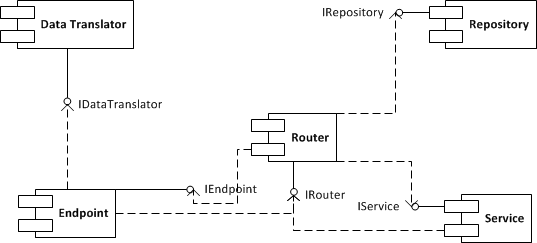
\includegraphics[scale=1.0]{component_uml.png}
	\caption{Diagram komponentów systemu SpeechProcessingPlatform w notacji UML 1.0}\label{fig:component_diagram}
\end{figure}

\section{Projekt}

Jak było wspomniane, do realizacji systemu SpeechProcessingPlatform została wybrana technologia ESB. Głównymi zaletami tej technologii są skalowalność i wysoki poziom abstrakcji, dzięki któremu budowa systemu jest ułatwiona - pozwala skupić się na problemie a nie na szczegółach implementacji. Dodatkowo, kontenery ESB dostarczają dużo użytecznych funkcjonalności takich jak: routing, transformacja danych, komunikacja oparta na wiadomościach, zestaw gotowych punktów końcowych. Wszystko to sprawia, że proces integracji jest znacznie ułatwiony. Projektowanie systemu z użyciem wiadomości jako modelu komunikacji, różni się od tradycyjnego podejścia z blokującymi wywołaniami metod. Interfejsy w postaci listy pól i metod, które dany komponent implementuje zostają zastąpione przez odpowiednie kanały wiadomości oraz format danych, które będą nimi przesyłane. Każdy komponent, który chce otrzymywać wiadomości udostępnia odpowiedni kanał pod dobrze znanym adresem, dzięki czemu inne komponenty są wstanie wysłać odpowiednie dla niego wiadomości. Dzięki użyciu tego modelu, zastosowanie dobrze sprawdzonych wzorców EIP staję się bardzo naturalne. 

\subsection{Warstwa \textit{Data Endpoints Layer}}

Ilustracja \ref{fig:endpoins_layer_project} przedstawia przepływ wiadomości w warstwie \textit{Data Endpoints Layer}. Aplikacje klienckie wysyłają żądanie przetwarzania na określony punkt końcowy, używając wybranego i obsługiwanego przez platformę protokołu. Żądania te zostają przetłumaczone na wspólny format wiadomości używany w dalszych częściach systemu, a następnie przesłane do routera. Dodatkowo, każdy punk końcowy posiada swój indywidualny kanał odpowiedzi, którego adres jest dodawany do wiadomości jako adres zwrotny. Dzięki temu, router będzie wstanie odesłać wynik przetwarzania do odpowiedniego punktu końcowego.

\begin{figure}[!h]
	\centering
	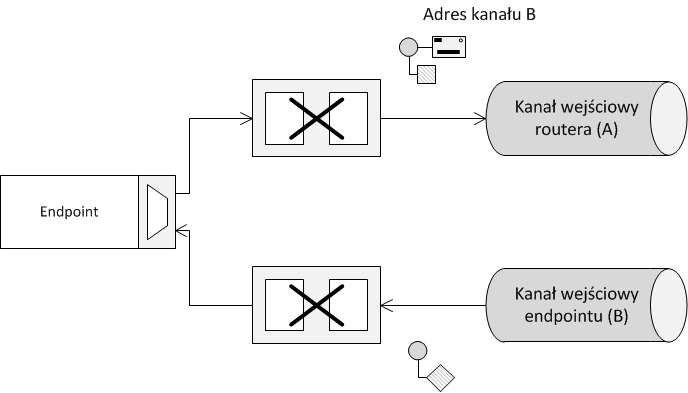
\includegraphics[scale=0.8]{endpoints_layer_flow.png}
	\caption{Diagram przepływu wiadomości w warstwie \textit{Data Endpoints Layer}}\label{fig:endpoins_layer_project}
\end{figure}

Ponieważ przetwarzanie mowy może być procesem czasochłonnym, budowana platforma powinna wspierać komunikację asynchroniczną. Niektóre punkty końcowe, takie jak FTP czy SMTP są z natury asynchroniczne. Aplikacja wykorzystująca protokół SMTP wysyła email z wymaganymi załącznikami na adres email punktu końcowego i wraca do swojego przetwarzania. Email zostaje odebrany przez platformę, następuje proces przetwarzania, a odpowiedź jest odsyłana na adres nadawcy. Gdy aplikacja odbierze email zwrotny może zacząć przetwarzanie odpowiedzi w dogodnym dla siebie czasie. Inne końcówki, takie jak REST czy SOAP, posiadają naturę synchroniczną, dlatego aby wspierały one komunikację asynchroniczną należy zastosować dodatkowe mechanizmy. W rozwiązaniu zastosowanym w platformie SpeechProcessingPlatform większość odpowiedzialności za dodanie obsługi asynchronicznej komunikacji spada na kolejne warstwy, dlatego zostanie ono dokładnie opisane w kolejnych podrozdziałach. Jedynym dodatkowym zadaniem punktów końcowych jest oznaczenie wiadomości jako przeznaczonej do przetwarzania asynchronicznego. Reszta procesu, z perspektywy punktu końcowego, nie ulega zmianie. Przy takim oznaczeniu, odpowiedź z warstwy routującej przychodzi bardzo szybko, lecz zawiera ona tylko identyfikator odpowiedzi, dzięki któremu aplikacja kliencka będzie mogła odpytać system czy jej zadanie zostało już zakończone. Takie zapytanie jest traktowane w taki sam sposób jak żądanie przetwarzania. Jeżeli zadanie zostało zakończone, wynik zostanie zwrócony aplikacji. Jeżeli nie, aplikacja będzie musiała wykonać zapytanie ponownie.

\subsection{Warstwa \textit{Routing Layer}}

\subsubsection*{Przepływ regularnych wiadomości}
Diagram \ref{fig:routing_layer_project} przedstawia, przepływ wiadomości, które zostały wysłane na adres warstwy routującej. Żądania, które już wcześniej były poddane transformacji, są gotowe aby wysłać je do odpowiednich serwisów. Komponent routujący, nie posiada stałych, wyznaczonych tras, lecz wybiera je za każdym razem gdy pojawi się jakaś wiadomość na jego kanale wejściowym. Jeżeli zadanie zostanie uznane za zakończone zostaje ono odesłane na adres zwrotny zapisany w wiadomości. Adres ten wskazuje kanał odbiorczy odpowiedniego punktu końcowego, za pomocą którego zostało zlecone dane zadanie przetwarzania. Jeżeli do zakończenia zadania potrzebny jest jeszcze jakiś etap przetwarzania, router wykonuje zapytanie do rejestru serwisów w celu uzyskania adresu serwisu spełniającego wymagania zadania. Jeżeli zostanie znaleziony odpowiedni serwis, żądanie przetwarzania zostaje opakowane w dodatkową kopertę, której adres zwrotny wskazuje na kanał wejściowy routera. Tak przygotowana wiadomość zostaje wysłana na adres uzyskany od rejestru serwisów. Po przetworzeniu, wiadomość jest odsyłana na adres wejściowy routera i jest podawana procesowi routowania ponownie. Jeżeli repozytorium nie zawiera serwisu spełniającego wymagania zadania, wiadomość jest odsyłana z powrotem do punktu końcowego z odpowiednim kodem błędu. 

\begin{figure}[!h]
	\centering
	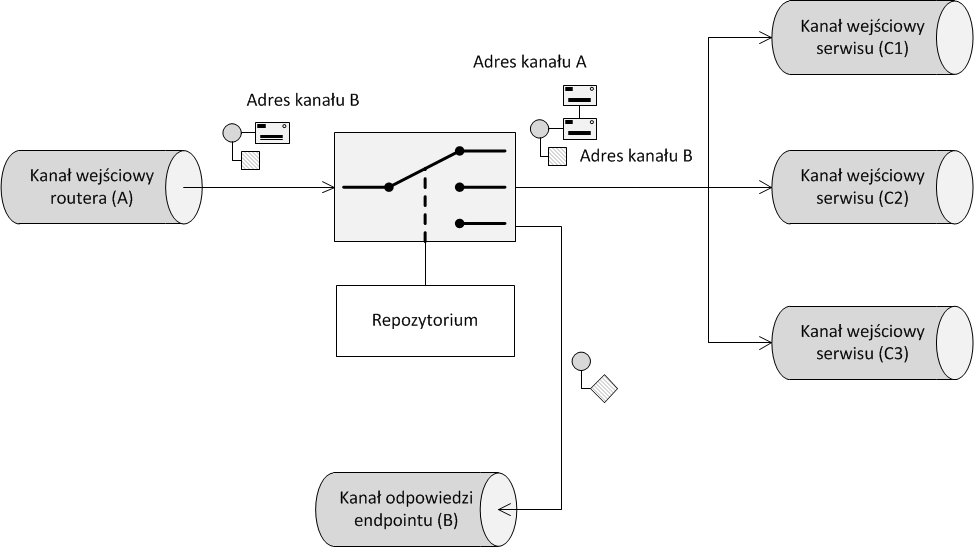
\includegraphics[scale=0.55]{router_flow.png}
	\caption{Diagram przepływu wiadomości w warstwie \textit{Routing Layer}}\label{fig:routing_layer_project}
\end{figure}

\begin{figure}[!h]
	\centering
	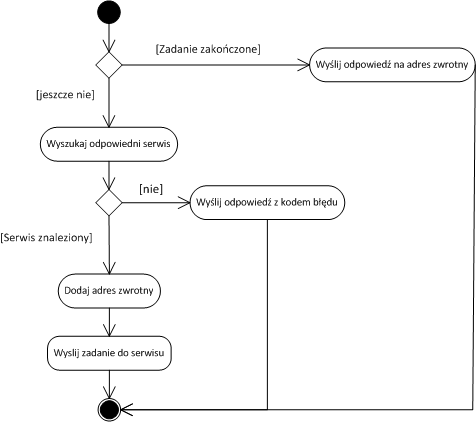
\includegraphics[scale=0.75]{router_activity.png}
	\caption{Diagram czynności komponentu routującego. }\label{fig:router_activity_diagram}
\end{figure}

\subsubsection*{Przepływ wiadomości asynchronicznych}
W celu obsługi wiadomości w sposób asynchroniczny, jeżeli wykorzystywany punkt końcowy nie zapewnia wparcia dla takiej komunikacji, należy poprzedzić proces routowania dodatkowymi krokami.
Diagram \ref{fig:asynchronous_detour} przedstawia rozwiązanie zastosowane w SpeechProcessingPlatform. Ważnym aspektem w prezentowanej koncepcji jest wprowadzenie dodatkowego typu serwisów, przechowywania danych, których zadaniem jest przechowywanie odpowiedzi pod odpowiednim kluczem. Pierwszym etapem jest rozdzielenie wiadomości na dwie grupy synchroniczne i asynchroniczne. Podział ten jest dokonywany na podstawie oznaczenia wykonanego przez punkt końcowy zlecający, a także na podstawie obecności chociaż jednego serwisu przechowywania danych. Jeżeli chociaż jeden z tych warunków nie jest spełniony żądanie będzie obsłużony w sposób opisany w poprzednim podrozdziale. Jeżeli obydwa warunki są spełnione wiadomość jest poddawana kilku dodatkowym operacjom przed wysłaniem jej do routera. Pierwsza z nich to usunięcie oznaczenia do przetwarzania asynchronicznego. Druga to wygenerowanie i dodanie do wiadomości unikalnego identyfikatora, który posłuży jako klucz przy przechowywaniu docelowej odpowiedzi. Następnym krokiem jest wygenerowanie zastępczej odpowiedzi i wysłanie jej do punktu końcowego. Odpowiedz ta zawiera wygenerowany wcześniej identyfikator, który pozwoli aplikacji klienckiej na odpytanie systemu o odpowiedź na oryginalne zadanie. Ostatnim krokiem jest podmiana adresu zwrotnego w oryginalnej wiadomości na adres serwisu przechowywania danych, do którego to odpowiedź zostanie wysłana po zakończonym przetwarzaniu.  Dalsze przetwarzanie wygląda tak samo jak w wypadku wiadomości synchronicznych.


 % mozna dodać obrazek do correlation idetifier po słowach : ...nagłówki: unikalny idetyfikator, oraz....

\begin{figure}[!h]
	\centering
	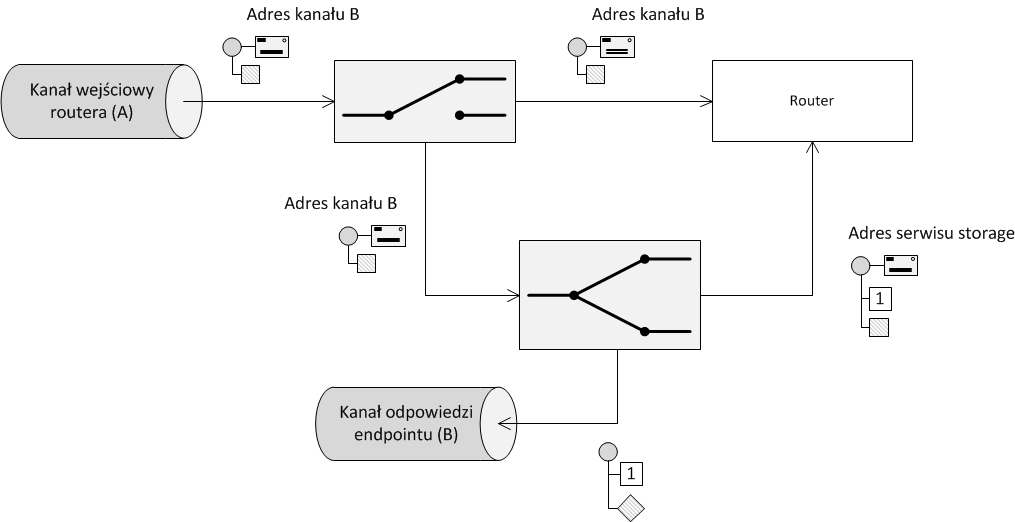
\includegraphics[scale=0.55]{asynchronous_detour.png}
	\caption{Diagram przepływu dla komunikacji asynchronicznej}\label{fig:asynchronous_detour}
\end{figure}

\begin{figure}[!h]
	\centering
	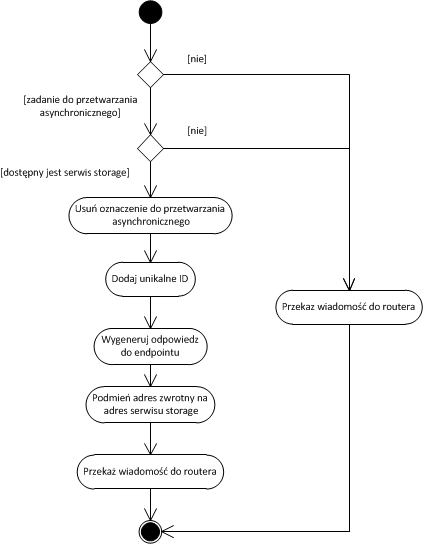
\includegraphics[scale=1.0]{asynchronous_activity_uml.png}
	\caption{Diagram czynności dla wiadomości asynchronicznych. }\label{fig:asynchronous_activity}
\end{figure}

\subsection{Warstwa \textit{Services Layer}}

Pierwszym komponentem z warstwy \textit{Services Layer}, który bierze udział podczas przetwarzania wiadomości jest repozytorium serwisów. Użycie tego komponentu nie jest wymagane , jednak jego brak wymusiłby zapisanie gdzieś w implementacji warstwy \textit{Routing Layer} stałych ścieżek lub zestawu reguł na podstawie których podejmowana byłaby decyzja o dalszej trasie wiadomości. Takie podejście mocno związałoby platformę z konkretnymi serwisami, dodanie nowego serwisu wiązało by się ze zmianą implementacji. Dzięki zastosowaniu repozytorium, które wprowadza dodatkową warstwę abstrakcji nad konkretnymi serwisami syntezy mowy, całość systemu nie jest związana z konkretnym dostawcą usług syntezy. Dodatkowym plusem takiego rozwiązania jest możliwość dynamicznego wyboru serwisów w zależności od zmieniających się warunków zewnętrznych. Platformę można rozszerzyć o komponenty monitorujące zachowanie się serwisów w czasie rzeczywistym co pozwoli na wybór najlepszej instancji w danym momencie. 
Aby nie wiązać platformy z konkretną implementacją repozytorium został wprowadzony interfejs, który musi być zaimplementowany przez komponenty chcące pełnić role repozytorium serwisów. Takie podejście pozwoli na użycie różnych implementacji opartych na rozmaitych technologiach jak np. Spring czy OSGi. Fragment kodu \ref{lst:repository_interface} przedstawia omawiany interfejs:

\lstset{language=Java, tabsize=4, caption=Definicja interfejsu ISreviceRepository w języku Java.,label=lst:repository_interface}

\begin{center}
\begin{lstlisting}
public interface SreviceRepository {
	Collection<String> lookupServicesURIs(Class type);
	Collection<String> lookupServicesURIs(Class type, Map<String, String> metaData);
	String lookupServiceURI(Class type);
	String lookupServiceURI(Class type, Map<String, String> metaData);
}
\end{lstlisting}
\end{center}

Chociaż repozytorium serwisów jest ważnym komponentem to nie bierze ono czynnego udziału w przetwarzaniu wiadomości. Adres serwisu który zostaje zwrócony jako odpowiedź na żądanie routera służy do wysłania zadania do odpowiedniej instancji serwisu. Diagram \ref{fig:services_layer_project} przedstawia przepływ wiadomości w warstwie \textit{Services Layer}. Przepływ ten jest stosunkowo prosty. Wiadomości pojawiające się w kanale wejściowym są odbierane i poddawane przetwarzaniu. Odpowiedź odsyłana jest na adres zwrotny zawarty w wiadomości, który zawsze wskazuje na adres kanału wejściowego routera. 

\begin{figure}[!h]
	\centering
	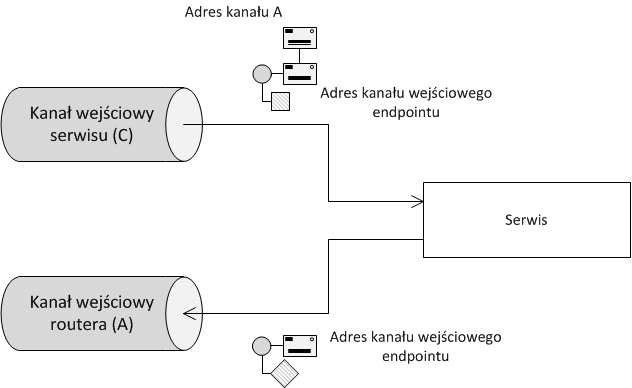
\includegraphics[scale=0.85]{services_layer_flow.png}
	\caption{Diagram przepływu wiadomości w warstwie \textit{Services Layer}}\label{fig:services_layer_project}
\end{figure}

Pierwszym wymaganiem stawianym konkretnym instancjom serwisów jest implementacja interfejsu \textit{MessageEnabledService} \ref{lst:service_interface}. Interfejs ten posiada tylko jedną metodę, która zwraca adres kanału wejściowego danego serwisu. Spełnienie tego wymagania jest konieczne aby repozytorium było w stanie odnaleźć serwis i zwrócić jego adres routerowi, jednak aby dana instancja pełniła jakąkolwiek rolę w systemie musi także udostępniać informację o funkcjonalności przez niej dostarczanej. W tym celu instancje muszą implementować dodatkowe interfejsy, które jednoznacznie określają udostępnianą funkcjonalność. Ponieważ komunikacja między serwisami, a resztą systemu odbywa się przez kanały wiadomości, interfejsy te służą tylko do oznaczenia serwisów a nie jako kontrakt miedzy nimi a, komponentami z nich korzystającymi. Takie użycie interfejsu jest znane jako wzorzec \textit{Marker interface} \cite{bloch2008}.

\lstset{language=Java, tabsize=4, caption=Definicja interfejsu MessageEnabledService w języku Java.,label=lst:service_interface}

\begin{center}
\begin{lstlisting}
public interface MessageEnabledService {
	String getServiceURI();
}
\end{lstlisting}
\end{center}

Jak było wspomniane wcześniej serwisy syntezy mowy zostały podzielone na 5 podstawowych grup, lecz nic nie stoi na przeszkodzie aby dodać kolejne, tak jak to ma miejsce z serwisami przechowywania danych. Jedyne co trzeba zrobić to zarejestrować serwis pod odpowiednim interfejsem. Fragment kodu \ref{lst:services_interfaces} przedstawia 5 interfejsów syntezy mowy plus interfejs serwisów przechowywania danych.

\lstset{language=Java, tabsize=4, caption=Definicja interfejsów serwisów w języku Java.,label=lst:services_interfaces}

\begin{center}
\begin{lstlisting}

public interface OCRService {
}

public interface TTSService {
}

public interface ASRService {
}

public interface TranslationService {
}

public interface LanguageRecognitionService {
}

public interface StorageService {
}
\end{lstlisting}
\end{center}

Drugim i ostatnim wymaganiem stawianym przed implementacjami serwisów jest obsługa wiadomości w wewnętrznym formacie używanym przez resztę komponentów systemu. Jest to spowodowane brakiem informacji na temat formatu wiadomości obsługiwanego przez dany serwis. Podczas procesu routowania, znany jest tylko adres i typ docelowego serwisu, dlatego router nie jest w stanie przetransformować wiadomości do obsługiwanego formatu. 


Większość dostępnych serwisów syntezy mowy nie była tworzona z myślą o obsłudze komunikacji opartej na wiadomościach, a nawet jeśli, to na pewno nie obsługują one formatu używanego w budowanym systemie. Aby możliwe było użycie gotowych serwisów w budowanym systemie należy użyć komponenty które będą działać na zasadzie proxy i to one będą rejestrować się w rejestrze serwisów. Po otrzymaniu wiadomości komponent proxy, podda ją wymaganej transformacji po czym wyśle zadanie do konkretnej instancji serwisu, używając przy tym odpowiedniego adaptera, jeżeli zajdzie taka potrzeba. 

\begin{figure}[!h]
	\centering
	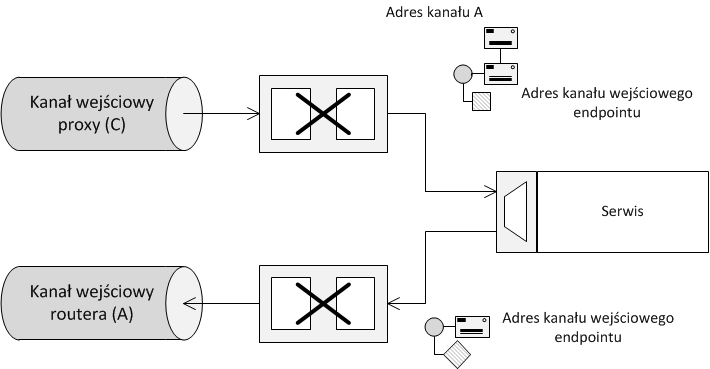
\includegraphics[scale=0.8]{proxy_layer_flow.png}
	\caption{Proxy wraz z elementami transformującymi oraz adapterem. }\label{fig:servis_proxy}
\end{figure}


\section{Implementacja}

Do implementacji systemu SpeechProcessingPlatform została użyta platforma integracyjna Apache ServiceMix, która w znaczący sposób ułatwia rozwiązywanie problemów integracji, dzięki dostarczaniu dużej ilości gotowych komponentów. Zastosowanie kontenera OSGi, na którym platforma ta jest oparta, pozawala na dynamiczną adaptację systemu w zależności od zaistniałych warunków. Dodatkowo pozwala podzielić system na niezależne, wymienialne części (bundle), z których każda posiada niezależny od reszty cykl życia. Dodawanie nowych części, takich jak kolejne punkty końcowe, czy kolejne serwisy może być realizowane w trakcie pracy systemu i nie wymaga jego ponownego uruchomienia \cite{hall2011}. 
Do implementacji przepływów wiadomości został użyty Apache Camel, który jest jedną z części składowych ServiceMix-a. Framework ten zawiera bardzo dużą liczbę wbudowanych punktów końcowych, obsługujących większość z popularnych protokołów komunikacji takich jak: FTP, HTTP, IMAP czy XMPP. Dzięki temu dodanie obsługi większej ilości protokołów nie stanowi żadnego problemu. Framework ten, pozwala również w prosty w sposób zaimplementować większość wzorców EIP, dlatego implementacja opisanych w poprzednim podrozdziale przepływów wiadomości jest stosunkowo prosta.

\subsection{Wewnętrzny format wiadomości}
Wiadomości przesyłane wewnątrz systemu mają postać obiektów, a pliki wejściowe są dołączone do nich jako załączniki. Takie podejście ułatwia operacje na wiadomościach, np. sprawdzenie czy zadanie jest już zakończone sprowadza się do wywołania metody. Fragment kodu \ref{lst:task_interface} przedstawia interfejs który musi być implementowany przez obiekty wiadomości.

\lstset{language=Java, tabsize=4, caption=Definicja interfejsu Task w języku Java.,label=lst:task_interface}

\begin{center}
\begin{lstlisting}
public interface Task {
	boolean isFinished();
	boolean isAsynchronous();
	Class getRequiredServiceType();
	Map<String, String> getMetaData();
	String getReturnAddress();
	void addReturnAddress(String address);
}
\end{lstlisting}
\end{center}

Zadania mogą mieć postać jedno lub wieloetapową, lecz fakt ten powinien być nie widoczny dla komponentów systemu. Jest to klasyczny przykład na zastosowanie wzorca projektowego kompozyt(diagram \ref{fig:composite_pattern}), który jest szeroko stosowany w informatyce, a szczegółowo opisany chociażby w \cite{gamma1995}.

\begin{figure}[!h]
	\centering
	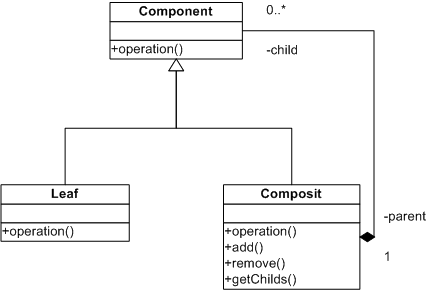
\includegraphics[scale=0.7]{composit_pattern.png}
	\caption{Wzorzec kompozyt}\label{fig:composite_pattern}
\end{figure}

Każdy z opisanych wcześniej rodzajów przetwarzania mowy posiada swoją klasę obiektów reprezentująca zadania danego typu. Diagram \ref {fig:task_class_hierarchy} przedstawia strukturę dziedziczenia klas reprezentujących obiekty zadań. Przedstawiona została tylko klasa zadań TTS, pozostałe klasy są analogiczne. 

\begin{figure}[!h]
	\centering
	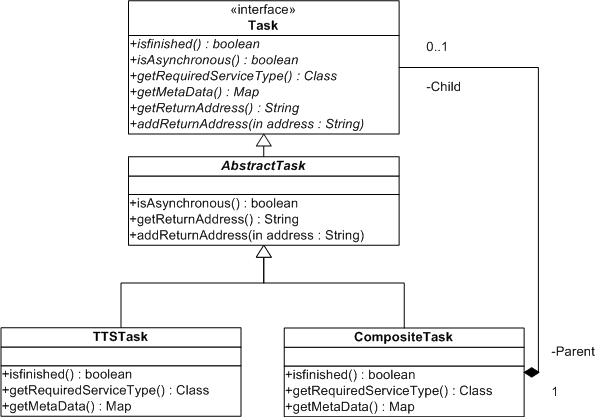
\includegraphics[scale=0.7]{tasks_hierarhy.png}
	\caption{Struktura dziedziiczenia klasy Task}\label{fig:task_class_hierarchy}
\end{figure}


\subsection{Warstwa \textit{Data Endpoints Layer}}

Dzięki bogatej bazie komponentów dostępnych w Apache Camel, implementacja konkretnych punktów końcowych sprowadza się raczej do konfiguracji. W większości przypadków jedyne co trzeba zrobić to dostarczyć odpowiedni adres URI, który pozwoli frameworkowi stworzyć i uruchomić wymagany punkt końcowy. Fragment kodu \ref{lst:camel_uris} przedstawia przykładowe formaty adresów URI

\lstset{language=Java, tabsize=4, caption=Przykładowe formaty adresów URI dla punktów końcowych Apache Camel.,label=lst:camel_uris}

\begin{center}
\begin{lstlisting}
	ftp://[username@]hostname[:port]/directoryname[?options]
	smtp://[username@]host[:port][?options]
	jms:[queue:|topic:]destinationName[?options]
	cxf:bean:cxfEndpoint[?options]
	cxfrs:bean:rsEndpoint[?options]
\end{lstlisting}
\end{center}

Aby użyć niektórych rodzajów punktów końcowych, wymagany nakład pracy jest trochę większy, lecz nadal stosunkowo mały. Chcąc udostępnić system za pomocą technologii Web services należało stworzyć również opis serwisu, jednak sprowadza się to do implementacji prostego interfejsu z dodatkowymi adnotacjami.  Fragment kodu \ref{lst:rest_service} przedstawia definicje serwisu REST-owego, która zastała użyta do konfiguracji punktu końcowego cxfrs. Metody w poniższej klasie nie są wywoływane, służą one tylko do konfiguracji punktu końcowego. Za całe przetwarzanie odpowiedzialna jest reszta ścieżki Apache Camel.


\lstset{language=Java, tabsize=4, caption=Definicja REST-owego punktu końcowego.,label=lst:rest_service}


%Trzeba to przejrzeć czy to działa zanim to sie pokaże wiekszej liczbie osób.
\begin{center}
\begin{lstlisting}
@Path("/speech_processing/rest")
public class RESTSpeechProcessingService {

	@POST
	@Path("/process")
    	public Response process(@FormParam("task")  String task, @FormParam("input")  File input) {
		return null;
	}

	@GET
	@PATH("/get_response")
	public Response getResponse(@QueryParam("id")  String responseId) {
		return null;
	}
}

\end{lstlisting}
\end{center}

Po odebraniu wiadomości przez punkt końcowy kolejnym krokiem jest jej transformacja do używanego wewnętrznie formatu. Wspieranie transformacji między różnymi formatami danych jest jednym z podstawowych wymagań stawianych przed rozwiązaniami ESB, dlatego też w ServiceMix-ie problem ten posiada bardzo duże wsparcie ze strony frameworku. Apache Camel udostępnia zbiór gotowych komponentów, dzięki którym transformacja między formatami takimi jak JSON, XML, czy CSV staje się trywialna. Jeżeli jednak, transformacja nie jest standardowa, framework posiada konstrukcje, które w łatwy sposób umożliwiają dodanie własnych komponentów transformujących. W przypadku transformacji wiadomości otrzymanych przez punkty końcowe, transformacja polega na zamianie opisu zadania w postaci pliku XML, na obiekt przedstawiający odpowiednie zadanie. Do tego zadania wykorzystano technologie JAXB \cite{jaxb2008}. Pozwala ona w prosty i przejrzysty sposób opisać mapowanie obiekt \begin{math}\Leftrightarrow\end{math} xml przy pomocy zestawu adnotacji. Dzięki zachowaniu odpowiedniej konwencji nazewnictwa opisanie mapowania sprowadza się do dodania tylko jednej adnotacji do każdej z klas opisujących zadania. Fragment kodu \ref{lst:jaxb_annotation} przedstawia klasę TTSTask z dodaną adnotacją JAXB.


% TO TEZ SPRAWDZIC , CZY ZADZIALA ZE ZLOZONYMI TYPAMI
\lstset{language=Java, tabsize=4, caption=Definicja klasy TTSTask wraz z adnotacjami JAXB .,label=lst:jaxb_annotation}

\begin{center}
\begin{lstlisting}
@XmlRootElement(name="tts")
public class TTSTask extends AbstarctTask {
	...
}
\end{lstlisting}
\end{center}

Ostatnim zadaniem punktu końcowego jest przesłanie gotowej wiadomości do routera. Jedyne czego do tego potrzebuje to adres URI kanału wejściowego routera. Adres ten jest dostarczany za pomocą pliku konfiguracyjnego. Takie rozwiązanie nie pozwala na dynamiczną zmianę ścieżki, lecz nie jest to wymagane ponieważ bez routera, reszta komponentów nie może pełnić swojej roli.
Fragment kodu \ref{lst:email_endpoint} przedstawia kompletną implementację przepływu wiadomości od punktu końcowego do routera.

\lstset{language=XML, tabsize=4, caption=Przykładowa\, kompletna implementacja przypływu wiadomości od punktu końcowego do routera przy pomocy XML DSL.,label=lst:email_endpoint}

\begin{center}
\begin{lstlisting}

<camelContext xmlns="http://camel.apache.org/schema/spring">

	<dataFormats>
		<jaxb id="jaxb" contextPath="pl.edu.agh.speechprocessing.tasks"/>
	</dataFormats>

	<route>
		<from uri="smtp://gmail.com?password=pass123&username=SpeechProcessingPlatform"/>
		<unmarshal ref="jaxb"/>
		<to uri="{{routerURI}}" />
	</route>

</camelContext>
\end{lstlisting}
\end{center}


\subsection{Warstwa \textit{Routing Layer}}

Najważniejszym elementem tej warstwy jak i całego systemu jest router. Jedyną zależnością pomiędzy routerem a innymi komponentami systemu jest jego adres, dzięki czemu system jest bardzo słabo powiązany z konkretną implementacją komponentu routującego, dzięki czemu implementacje te można dowolnie podmieniać stosownie do zaistniałych potrzeb. Apache Camel bardzo upraszcza proces implementacji routera. Dzięki użyciu elementu \textit{dynamicRouter} jedyne co zostaje do implementacji to metoda zwracająca odpowiedni adres URI. Ponieważ \textit{dynamicRouter} musi być ostatnim elementem ścieżki, ustawienie poprawnego adresu zwrotnego musi zostać podzielone na dwa etapy. Pierwszy etap następuje przed etapem routowania i polega na dodaniu adresu zwrotnego routera niezależnie od tego gdzie ostatecznie wiadomość zostanie przesłana. Drugi etap polega na usunięciu adresu routera z wiadomości i następuje tylko jeżeli proces przetwarzania został zakończony, czyli jeżeli wszystkie wymagane kroki zostały wykonane albo któryś z nich nie może zostać wykonany z powodu braku odpowiedniego serwisu. Poniżej przedstawiona została przykładowa ścieżka Apache Camel odpowiadająca za przepływ wiadomości w opisywanej warstwie jak i przykładowa implementacja komponentu routującego.

\lstset{language=XML, tabsize=4, caption=Scieżka Apache Camel odpowiadająca za przepływ wiadomości w warstwie \textit{Routing Layer}.,label=lst:routin_layer_impl}

%SPRAWDZIĆ
\begin{center}
\begin{lstlisting}
<bean id="dynamicRouter" class="pl.edu.agh.speechprocessing.routing.DynamicRouter"/>

<camelContext xmlns="http://camel.apache.org/schema/spring">

	<route>
		<from uri="{{routerURI}}" />
		<bean ref="dynamicRouter" method="addRouterAddress"/>
		<dynamicRouter>
			<method ref="dynamicRouter" method="route" />
		</dynamicRouter>
	</route>

	<route>
		<from uri="direct:responseChannel">
		<bean ref="dynamicRouter" method="removeRouterAddress"/>
		<dynamicRouter>
			<method ref="dynamicRouter" method="routeResponse" />
		</dynamicRouter>
	</route>

</camelContext>

\end{lstlisting}
\end{center}

\lstset{language=Java, tabsize=4, caption=Implementacja metody routującej wiadomości do odpowiednich serwisów.,label=lst:router_impl}

\begin{center}
\begin{lstlisting}

class DynamicRouter {

	...

	public String route(Task task) {
		if (task.isFinished()) {
			return "direct:responseChannel";
		} else {
			String uri = serviceRepository.lookupServiceURI(task.getRequiredServiceType(), task.getMetaData());
			if (service != null) {
				return uri;
			} else {
				return "direct:responseChannel";
			}
		}
	}

	public String routeResponse(Task task) {
		return task.getReturnAddress();
	}

	public Task removeRouterAddress(Task task) {
		//usuniecie adresu routera z listy adresow zwrotnych
		task.getReturnAddress();
		return task;
	}

	public Task addRouterAddress(Task task) {
		task.addReturnAddress(getRouterAddress());
		return task;
	}

	...
end
\end{lstlisting}
\end{center}

\subsection{Warstwa \textit{Services Layer}}

Implementacja repozytorium serwisów zastosowana w systemie SpeechProcessingPlatform jest oparta na technologii OSGi, lecz dzięki dobrze wyspecifikowanemu interfejsowi, system ten nie jest związany z tą jedną, konkretną implementacją. Bazowanie na kontenerze OSGi pozwala dodać dynamiczną naturę do systemu. Takie podejście pozwala dodawać nowe serwisy bez zatrzymywania systemu. Ponieważ OSGi posiada wbudowany rejestr serwisów, więc cała logika związana z rejestrowaniem się i utrzymywaniem listy dostępnych serwisów jest zapewniona, jedyne co zostaje do zaimplementowania to proces odpytywania rejestru o odpowiedni serwis. Podstawowym typem wyszukiwania jakie udostępnia rejestr OSGi jest wyszukiwanie po typie serwisu. Dodatkowo udostępnia on metodę wyszukiwania, która przyjmuje standardowy filtr LDAP \cite{ldaprfc1996} w postaci ciągu znaków. Rejestr OSGi porównuje parametry z filtru z parametrami w definicji serwisu i na tej podstawie podejmuje decyduję które referencje do serwisów zwrócić. Fragment \ref{lst:ldap_tts_query} przedstawia przykładowe zapytanie LDAP zawierające parametry dotyczące przetwarzania mowy. Oprócz opisu serwisów w postaci typu oraz parametrów, OSGi pozwala również na nadawanie im rankingu, dzięki czemu jeżeli więcej niż jeden serwis spełnia zadane wymagania, pozwala zdecydować który serwis jest lepszy. Kompletny algorytm wyboru najlepiej pasującego serwisu można znaleźć w \cite{hall2011}. Fragment kodu \ref{lst:service_repository_impl} przedstawia klasę OSGIServiceRepository, która pełni funkcję fasady nad rejestrem wbudowanym w OSGi.

\lstset{language=Java, tabsize=4, caption=Przykładowe zapytanie LDAP zawierające parametry dotyczące serwisu TTS ,label=lst:ldap_tts_query}

\begin{center}
\begin{lstlisting}

//zapytanie o serwis TTS
"(&(language=en)(codec=mp3))"

/zaptanie o serwis OCR
"(&(language=pl)(|(imageFormat=jpg)(imageFormat=jpeg)))"


\end{lstlisting}
\end{center}

\lstset{language=Java, tabsize=4, caption=Częściowa definicja klasy OSGIServiceRepository będącą fasadą nad Rejestrem OSGi. ,label=lst:service_repository_impl}

\begin{center}
\begin{lstlisting}
public class TTSTask implements SreviceRepository{
	private BundleContext bundleContext;
	...
	
	public Collection<String> lookupServicesURIs(Class type) {
		ServiceReference[] refList = bundleContext.getServiceReferences(type.getName())
		return prepareURIsList(refList);
	}

	public Collection<String> lookupServicesURIs(Class type, Map<String, String> metaData) {
		ServiceReference[] refList = bundleContext.getServiceReferences(type.getName(), preapreFilterQuery(metaData));
		return prepareURIsList(refList);
	}

	...
}

\end{lstlisting}
\end{center}
% MOZNA DODAC REFERENCJE DO LBUEPRINTA
Ostatnimi elementami systemu są konkretne serwisy, jednak aby jakiś serwis mógł zostać użyty w systemie musi spełniać parę warunków. Pierwszyw warunkiem jest umiejętność obsługi wiadomości co jest równoznaczne z udostępnianiem jakiegoś kanału wejściowego, który pozwoli na komunikącje routera z daną implementacją. Drugim warunkiem jest rejestracja w rejestrze OSGi pod odpowiednimi interfejsami oraz z odpowiednimi parametrami, co pozwoli na wyszukanie serwisu podczas procesu routowania. W celu rejestracji serwisów został użyty kontener Blueprint, który jest dostarczony razem z frameworkiem OSGi. Pozwala on na łatwą i przejrzystą definicję serwisów za pomocą plików konfiguracyjnych w formacie xml. Oprócz tego, pozwala on również na definicję oraz wstrzykiwanie zależności co upraszcza konfiguracje systemu. Fragment kodu \ref{lst:blueprint_definition} przedstawia definicje serwisu OCR przy uzyciu kontenera Blueprint.

\lstset{language=XML, tabsize=4, caption=Definicja serwisu OCR przy użyciue kontenera Blueprint.,label=lst:blueprint_definition}

%SPRAWDZIĆ
\begin{center}
\begin{lstlisting}
<blueprint xmlns="http://www.osgi.org/xmlns/blueprint/v1.0.0">

	 <!-- definicja beanu ktory zostanie zarejestrowany jako serwis, jako argument przyjmuje nazwe kanalu wejsciowego -->
	<bean id="freeOCRServiceImpl" class="pl.edu.agh.speechprocessing.services.FreeOCRService">
		 <argument value="direct:freeOCRService"/> 
	</bean>

	<service ref="freeOCRService" auto-export="interfaces" ranking="5">
		<service-properties>
			<entry key="language">
				<set value-type="java.lang.String">
					<value>en</value>
					<value>it</value>
					<value>pl</value>
				</set> 
			</entry>
			<entry key="imageFormat">
				<set value-type="java.lang.String">
					<value>bmp</value>
					<value>png</value>
					<value>jpg</value>
				</set> 
			</entry>
		</service-properties>
	</service>

</blueprint>

\end{lstlisting}
\end{center}

Serwisy rejestrowane w rejestrze OSGi pełnią tylko pomocniczą role. Ich zadaniem jest umożliwienie wyszukiwania oraz dostarczanie adresu pod który należy wysłać wiadomość do zainteresowanych routera. Całe przetwarzanie zaczyna się po otrzymaniu wiadomości w kanale odbiorczym udostępnianym przez dany serwis. Oczywiście obiekt, który jest rejestrowany może również brać czynny udział w przetwarzaniu, ale nie musi. Jako ża właściwe serwisy, które dokonują przetwarzania są na zewnątrz systemu, jedyne zadanie jakie pozostaje to przyogotwanie wiadomości, wywołanie serwisu używając odpowiedniego protokołu, przetłumaczenie odpowiedzi na format wewnętrzny i odesłanie jej do routera. 


% Można dodać fragment implementacji.

\section*{Podsumowanie} 

Powyższy rozdział przedstawił projekt i implementację przykładowej platformy integracyjnej dla przetwarzania mowy. Zastosowanie architekryury z luźno powiązanymi warstwami zostawia dużo opcji do przyszłego rozwoju systemu. Prezentowany system jest też przykładem na to jak użycie wyspecjalizowanych technologii upraszcza proces integracji. Apache ServiceMix integrujący w sobie takie technologie jak OSGi czy Apache Camel pozwala budować systemu integracyjne z gotowych elementów pozwalając ich twórcom skupić sie na logice przypływu danych. Zaimplementowany system należy poddać weryfikacji względem wymagań postawionych w rozdziale 2, a także sprawdzić jego wydajność w porównaniu z tradycyjnym podejściem do systemów przetwarzania mowy.


% można wrzucic obrazek całego systemu

%Jednym z rozwiązań jest użycie wzorca \textit{Correlation Identifier}\cite{eaipatterns}:

%\begin{figure}[!h]
%	\centering
%	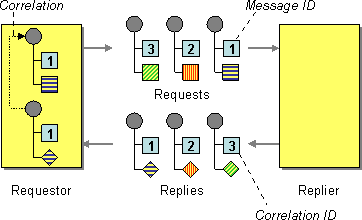
\includegraphics{CorrelationIdentifierSolution.png}
%	\caption{Wzorzec \textit{Correlation Identifier}: \url{http://www.eaipatterns.com/img/CorrelationIdentifierSolution.gif}}\label{fig:correlation_identifier}
%\end{figure}

%Endpoint po otrzymaniu żądania generuje dla niego unikalny identyfikator, który odsyła aplikacji nie czekając na wynik przetwarzania. Ten sam identyfikator jest dodawany do wiadomości %wysyłanej do routera, lecz tym razem adres zwrotny wskazuje nie na punkt końcowy lecz na serwis 



% rysunek z podziałęm na komponenty,
% rysunek EIP - ale to może być już w projekcie.
% proekt, interfejsy, chierarchie klas. 









% ---------------------------------------------------------------------------
%: ----------------------- end of thesis sub-document ------------------------
% ---------------------------------------------------------------------------



% this file is called up by thesis.tex
% content in this file will be fed into the main document

\chapter{Podsumowanie} % top level followed by section, subsection


% ----------------------- paths to graphics ------------------------

% change according to folder and file names
\ifpdf
    \graphicspath{{7/figures/PNG/}{7/figures/PDF/}{7/figures/}}
\else
    \graphicspath{{7/figures/EPS/}{7/figures/}}
\fi

Obecnie istnieje bardzo dużo róznych serwisów oferujących przetwarzanie mowy. Jednak ich poważną wadą jest to, że dziedzina ich pracy jest bardzo wąska. Brakuje systemów oferujących więcej niż jeden sposób transformacji. Autorzy tej pracy starali się sprawdzic czy integracja takich systemów jest dobrym pomysłem oraz jeżeli tak to jakie podejście jest najlepsze. Jak zostało to zaprezentowane w powyższych rozdziałach stworzenie systemu integrującego serwisy posiadające różne funkcje ma dużo zalet i bardzo ułatwia tworzenie aplikacji wykorzystujących te serwisy. Co więcej dodatkowa warstwa abstrakcji, która powstaje w ten sposób, nie wpływa w sposób znaczący na szybkość działania aplikacji klienckich (w porównaniu z sytuacją w której aplikacja kliencka sama musiałaby komunikować się z tymi serwisami). Wszystko to wyraźnie pokazuje, że istnienie takiego zintegrowanego serwisu ma sens i jest na niego zapotrzebowanie. \\
Co do wyboru sposobu integracji, jak zostało to zaprezentowane wyżej istnieje wiele odrębnych sposobów, z których każdy ma swoje zalety i wady. Po dogłębnej analizie dostępnych rozwiązań integracyjnych autorzy pracy zdecydowali, że najlepszy efekt daje najnowsze rozwiązanie a więc ESB. Posiada ono szereg zalet które należy uwypuklić:
\begin{itemize}
	\item Łatwość rozbudowy - gdy powstanie jakiś nowy serwis, oferujący ciekawą funkcjonalność jedynym wysiłkiem jaki należy wykonać w celu użycia go, jest wpięcie serwisu do szyny
	\item Lekkość - warstwa abtrakcji nakładana przez ESB w celu połączenia dostępnych serwisów jest bardzo mała i nie ma wpływu na wydajność
	\item Skalowalność - różne instancje ESB mogą łączyć się razem w celu uzyskania wyższej wydajności oraz rozproszenia geograficznego
	\item Różnorodność - wszystkie istniejące implementacje ESB oferują wiele różnych endpoint'ów, służących jako interfejsy wejścia/wyjścia, obsługujących wiele formatów
\end{itemize}
Wykorzystanie takiego podejścia daje też inny duży, plus jakim niewątpliwie jest łatwość ukrywania implementacji. Klienci systemu opartego na takim rozwiązaniu nie będą wiedzieć z jakich konkretnie serwisów korzystają, przez co w razie wystąpienia kłopotów czy też pojawienia się nowszego, lepszego lub ciekawszego rozwiązania można taki serwis łatwo podmienić, bez konieczności zmieniania API. Kolejną dużą zaletą wykorzystania ESB, jest możliwość wykorzystania routingu. Dzięki temu sterowanie całym systemem i kolejnością wywoływania poszczególnych serwisów jest możliwa za pomocą prostego pliku xml.  \\
Zaprezentowana praca magisterska zagłębia się w dziedzinę, która jest dość nowatorska. Zaproponowane rozwiązanie i przykładowa implementacja pokazują zarówno, iż temat jest ciekawy i warty dalszych badań oraz, że istniejące w tej chwili rozwiązania integracyjne są odpowiednie dla specyficznej dziedziny jaką jest przetwarzanie mowy i można je z powodzeniem stosować. 

% ----------------------- contents from here ------------------------






% ---------------------------------------------------------------------------
% ----------------------- end of thesis sub-document ------------------------
% ---------------------------------------------------------------------------               % discussion of results

%
% this file is called up by thesis.tex
% content in this file will be fed into the main document

\chapter{Materials \& methods} % top level followed by section, subsection


% ----------------------- paths to graphics ------------------------

% change according to folder and file names
\ifpdf
    \graphicspath{{8/figures/PNG/}{8/figures/PDF/}{8/figures/}}
\else
    \graphicspath{{8/figures/EPS/}{8/figures/}}
\fi

% ----------------------- contents from here ------------------------




 

% ---------------------------------------------------------------------------
%: ----------------------- end of thesis sub-document ------------------------
% ---------------------------------------------------------------------------



 






        % description of lab methods




% --------------------------------------------------------------
%:                  BACK MATTER: appendices, refs,..
% --------------------------------------------------------------

% the back matter: appendix and references close the thesis


%: ----------------------- bibliography ------------------------

% The section below defines how references are listed and formatted
% The default below is 2 columns, small font, complete author names.
% Entries are also linked back to the page number in the text and to external URL if provided in the BibTex file.

% PhDbiblio-url2 = names small caps, title bold & hyperlinked, link to page 
%\begin{multicols}{1} % \begin{multicols}{ # columns}[ header text][ space]
%\begin{tiny} % tiny(5) < scriptsize(7) < footnotesize(8) < small (9)

\bibliographystyle{Latex/Classes/PhDbiblio-url2} % Title is link if provided
\renewcommand{\bibname}{Bibliografia} % changes the header; default: Bibliography

\bibliography{9_backmatter/references} % adjust this to fit your BibTex file

%\end{tiny}
%\end{multicols}

% --------------------------------------------------------------
% Various bibliography styles exit. Replace above style as desired.

% in-text refs: (1) (1; 2)
% ref list: alphabetical; author(s) in small caps; initials last name; page(s)
%\bibliographystyle{Latex/Classes/PhDbiblio-case} % title forced lower case
%\bibliographystyle{Latex/Classes/PhDbiblio-bold} % title as in bibtex but bold
%\bibliographystyle{Latex/Classes/PhDbiblio-url} % bold + www link if provided

%\bibliographystyle{Latex/Classes/jmb} % calls style file jmb.bst
% in-text refs: author (year) without brackets
% ref list: alphabetical; author(s) in normal font; last name, initials; page(s)

%\bibliographystyle{plainnat} % calls style file plainnat.bst
% in-text refs: author (year) without brackets
% (this works with package natbib)


% --------------------------------------------------------------

% according to Dresden med fac summary has to be at the end
%
% Thesis Abstract -----------------------------------------------------

%\begin{abstractslong}    %uncommenting this line, gives a different abstract heading
\begin{abstracts}        %this creates the heading for the abstract page

Rozwój technologiczny, a w szczególności rozwój komputerów i technologii z nimi związanych w ciągu ostatnich lat jest bardzo szybki. Zmieniają się zarówno, podzespoły, moc obliczeniowa, rozmiary, wygląd a nawet interfejsy. Komputery wkroczyły, lub są temu bardzo bliskie, do niemal każdej dziedziny życia. W związku z tym zmienia się sposób komunikacji między użytkownikiem a komputerem. W ostatnich czasach można zaobserwować dążenie inżynierów i projektantów do uczynienia komunikacji z komputerem jak najbardziej naturalną. Pomysły są różne od "kontrolerów bez kontrolera" jak Microsoft Kinect \footnote {http://www.xbox.com/en-US/kinect}, poprzez rozwiązania "ruchowe" podobne do tego na jakie zdecydowało się Sony \footnote{http://www.sony.com/} w swoim kontrolerze PlayStation Move \footnote{http://us.playstation.com/ps3/playstation-move/} poprzez klasyczne  jak mysz i klawiatura. Jednak najbardziej naturalnym sposobem porozumiewania się wydaje się głos. Najbardziej znanym, bo napewno nie pionierskim, systemem który komunikuję się z użytkownikiem za pomocą głosu jest Apple Siri \footnote{http://www.apple.com/iphone/features/siri.html} - osobisty asystent, "żyjacy" wewnątrz systemu, umożliwiający dostęp do jego funkcji za pomocą mowy.\\
Niniejsza praca przedstawia prototyp systemu UniversalSynthesizer, służacego do zamiany tekstu na dźwięk i mowy na tekst, będącego zaawansowaną, rozproszoną, rozszerzalną, wielojęzyczną platformą/serwisem umożliwiającą łatwe tworzenie zróżnicowanych, wieloplatformowych aplikacji, mających różne zadania. Celem pracy nie było stworzenie gotowego do użytku, kompletnego, w pełni sprawnego produktu. Powstałą aplikację należy traktować bardziej jako punkt wyjścia, prototyp który w przyszłości może być wykorzystany do zbudowanie w pełni funkcjonalnego, ogólnie dostępnego, komercyjnego lub otwartego systemu. W związku z tym niektóre zagadnienia, dość istotne z punktu widzenia potencjalnego odbiorcy, ale nie będące ściśle powiązane z celem pracy zostały pominięty lub też niedopracowane. 
\end{abstracts}
%\end{abstractlongs}


% ---------------------------------------------------------------------- 



%: ----------------------- list of figures/tables ------------------------

\listoffigures	% print list of figures
\renewcommand{\lstlistlistingname}{Spis fragmentów kodu}
\lstlistoflistings
\addcontentsline{toc}{chapter}{Spis fragmentów kodu}

%\listoftables  % print list of tables

\lstset{language=XML, tabsize=4,caption=XML Schema dla pliku konfiguracyjnego,label=lst:xml_schema}
\appendix
\chapter{XML Schema dla pliku konfiguracyjnego}
\lstset{caption={Plik konfiguracyjny xml},label=DescriptiveLabel}
\begin{lstlisting}
\caption{Model "Hub and spoke"}\label{fig:hub_and_spoke}
<?xml version="1.0" encoding="utf-8"?>
<xs:schema elementFormDefault="qualified" xmlns:xs="http://www.w3.org/2001/XMLSchema">
	<xs:element name="speechProcessingInstructions">
		<xs:complexType>
			<xs:sequence>
				<xs:element name="readImage" type="xs:string" default="" minOccurs="0"/>
				<xs:element name="identifyLanguage" type="xs:string" default="" minOccurs="0"/>
				<xs:element name="translate" minOccurs="0">
					<xs:complexType>
						<xs:sequence>
							<xs:element name="inputLanguage" type="xs:string" default="polish" minOccurs="0" />
							<xs:element name="outputLanguage" type="xs:string" default="polish"/>
						<xs:sequence>
					</xs:complexType>
				</xs:element>
				<xs:element name="performTTS" type="languageInfo" minOccurs="0"/>
				<xs:element name="performASR" type="languageInfo" minOccurs="0"/>
			</xs:sequence>
		</xs:complexType>
	</xs:element>
			
	<xs:complexType name="languageInfo">
		<xs:sequence>
			<xs:element name="language" type="xs:string"/>
		</xs:sequence>
	</xs:complexType>
	
</xs:schema>

\end{lstlisting}
\end{document}
